\documentclass[12pt,oneside]{report}

\usepackage[letterpaper,margin=1in]{geometry}
\usepackage{amsmath}
\usepackage{array}
\usepackage{booktabs}
\usepackage{caption}
\usepackage{etoolbox}
\usepackage{listings}
\usepackage[nopatch=footnote]{microtype}
\usepackage{needspace}
\usepackage{ragged2e}
\usepackage{setspace}
\usepackage{tabularx}
\usepackage{tikz}
\usepackage{xcolor}
\usepackage{xurl}
\usepackage{hyperref}
\usetikzlibrary{arrows.meta,calc,decorations.pathreplacing,fit,matrix,positioning}

\onehalfspacing

\newcommand{\einlang}{\textsc{Einlang}}
\newcommand{\pathcode}[1]{\nolinkurl{#1}}
\newcolumntype{L}[1]{>{\RaggedRight\arraybackslash}p{#1}}
\newcolumntype{Y}{>{\RaggedRight\arraybackslash}X}
\emergencystretch=2em

\definecolor{einKeyword}{RGB}{0,74,128}
\definecolor{einComment}{RGB}{90,104,120}
\definecolor{einString}{RGB}{153,79,0}
\definecolor{einFrame}{RGB}{188,194,201}
\definecolor{einBg}{RGB}{249,250,251}
\definecolor{figInk}{RGB}{29,44,61}
\definecolor{figLine}{RGB}{122,136,150}
\definecolor{figBlue}{RGB}{39,92,138}
\definecolor{figBlueBg}{RGB}{235,244,250}
\definecolor{figGreen}{RGB}{55,111,92}
\definecolor{figGreenBg}{RGB}{233,244,239}
\definecolor{figGold}{RGB}{167,116,39}
\definecolor{figGoldBg}{RGB}{250,244,230}
\definecolor{figRose}{RGB}{155,83,71}
\definecolor{figRoseBg}{RGB}{248,238,234}
\definecolor{figSlateBg}{RGB}{243,246,248}

\hypersetup{
  colorlinks=true,
  linkcolor=einKeyword,
  citecolor=einKeyword,
  urlcolor=einKeyword,
  linktoc=all,
  bookmarksnumbered=true,
  bookmarksopen=true
}
\Urlmuskip=0mu plus 2mu

\lstdefinelanguage{Einlang}{
  morekeywords={let,fn,if,else,match,use,where,sum,in,assert,print,true,false,as},
  sensitive=true,
  morecomment=[l]{//},
  morestring=[b]"
}

\lstdefinestyle{einlang}{
  language=Einlang,
  basicstyle=\ttfamily\footnotesize,
  keywordstyle=\color{einKeyword}\bfseries,
  commentstyle=\color{einComment}\itshape,
  stringstyle=\color{einString},
  breaklines=true,
  breakatwhitespace=true,
  columns=fullflexible,
  keepspaces=true,
  frame=single,
  framerule=0.4pt,
  rulecolor=\color{einFrame},
  backgroundcolor=\color{einBg},
  framesep=4pt,
  showstringspaces=false,
  aboveskip=0.4\baselineskip,
  belowskip=0.4\baselineskip
}

\lstdefinestyle{pythoncode}{
  language=Python,
  basicstyle=\ttfamily\footnotesize,
  keywordstyle=\color{einKeyword}\bfseries,
  commentstyle=\color{einComment}\itshape,
  stringstyle=\color{einString},
  breaklines=true,
  breakatwhitespace=true,
  columns=fullflexible,
  keepspaces=true,
  frame=single,
  framerule=0.4pt,
  rulecolor=\color{einFrame},
  backgroundcolor=\color{einBg},
  framesep=4pt,
  showstringspaces=false,
  aboveskip=0.4\baselineskip,
  belowskip=0.4\baselineskip
}

\BeforeBeginEnvironment{lstlisting}{\par\Needspace{12\baselineskip}}

\title{\einlang{}: A Source Language for Indexed Tensor Programs with Recurrence and Local Derivatives}
\author{Bowen Fu}
\date{April 2026}

\begin{document}

\hypersetup{pageanchor=false}
\begin{titlepage}
\centering
\vspace*{1.0in}
{\Large \einlang{}: A Source Language for Indexed Tensor Programs with Recurrence and Local Derivatives\par}
\vspace{0.75in}
{\large Bowen Fu\par}
\vfill
{\large A thesis-form project report\par}
\vspace{0.3in}
{\large April 2026\par}
\end{titlepage}
\clearpage
\hypersetup{pageanchor=true}

\pagenumbering{roman}

\chapter*{Abstract}
\addcontentsline{toc}{chapter}{Abstract}

Tensor programs need a source boundary that users can write directly and
compilers can inspect. A common pattern still crosses several boundaries:
multidimensional indexing, recurrent state updates, and sensitivity queries are
usually expressed through separate interfaces such as \texttt{einsum}-like
functions, host-language loops or scan combinators, and \texttt{grad} or
\texttt{backward} APIs. This fragmentation makes programs executable, but it
hides the source facts that connect the mathematical definition to compiler
analysis.

This thesis presents \einlang{}, a tensor language and compiler that integrates
multidimensional indexed definitions, declarative recurrences, and local
derivative requests in one binding environment. In \einlang{}, a recurrence is a
named binding over an index space that declares its dependencies; later
expressions can read points of that recurrence, and derivative requests can
target either final results or intermediate bindings. The contribution is an
executable abstraction boundary: indexed clauses define axes and covered
domains, recurrent bindings define dependency graphs, and derivative requests
denote shaped derivative values.

The thesis also documents the non-trivial implementation pieces that make this
boundary executable: the grammar and transformer front end, DefId-based name
resolution, module loading and standard-library discovery, the IR and pass
pipeline, range and shape analyses, type inference and monomorphization,
Einstein lowering, recurrence ordering and storage metadata, compile-time and
runtime autodiff machinery, NumPy execution, the experimental IREE backend,
diagnostics, testing, and example validation. The result is a source form for
tensor programs that stays close to the mathematical description while
preserving structure for compiler and runtime passes.


\cleardoublepage
\phantomsection
\pdfbookmark[0]{Contents}{toc}
\tableofcontents
\clearpage
\pagenumbering{arabic}

\chapter{Introduction}

Programs for machine learning, simulation, optimization, and dynamic programming
are often written as tensor equations. The programmer names axes, sums over
intermediate dimensions, carries state through a recurrence, and eventually asks
how one quantity changes with respect to another. Those activities are
mathematically related, but contemporary programming systems often expose them
through separate interfaces.

For example, a computation may use an \texttt{einsum} string to express a
contraction, a host-language loop or scan combinator to express recurrence, and
a separate automatic-differentiation transform to obtain a gradient. The program
executes, but the compiler-facing facts are scattered: output axes are hidden in
one notation, recurrence dependencies in another, and derivative targets in a
third. The central question of this thesis is whether those facts can remain in
one source language without sacrificing executable behavior.

\section{Thesis Statement}

The thesis is that indexed tensor definitions, declarative recurrence, and local
derivative requests form a productive abstraction boundary for tensor-heavy
programs. When these constructs share one binding environment, the source
program keeps mathematical structure visible long enough for compiler passes to
check shape consistency, derive recurrence order, choose storage windows, and
lower derivative requests as shaped values.

\section{Implementation Scope}

This document is intentionally broader than the paper. The paper isolates the
language-design claim. The thesis treats \einlang{} as an implementation
artifact and documents the substantial subsystems in the repository:

\begin{table}[htbp]
\centering
\caption{Implementation subsystems covered by this thesis.}
\label{tab:implementation-map}
\renewcommand{\arraystretch}{1.08}
\begin{tabular}{@{}L{0.32\textwidth}L{0.56\textwidth}@{}}
\toprule
Subsystem & Non-trivial responsibility \\
\midrule
Frontend & Lark grammar, parse caching, source locations, AST construction, string interpolation, functions, literals, patterns, and Einstein syntax. \\
Identity and modules & DefId allocation, scoped resolution, Rust-like module paths, stdlib discovery, imports, aliases, re-exports, and Python module hooks. \\
IR and passes & Slot-based IR nodes, visitors, S-expression serialization, pass ordering, \texttt{TyCtxt}, range, shape, type, validation, pruning, lowering, and tree shaking. \\
Tensor lowering & Einstein declaration grouping, rest-index preprocessing, implicit range discovery, lowerings for reductions, selections, comprehensions, and backend execution facts. \\
Recurrence & Dependency extraction, recurrence-dimension ordering, same-timestep dependencies, storage-window metadata, and circular-buffer runtime execution. \\
Autodiff & Source \texttt{@} forms, differential IR, high-level differentiation, request lowering, leak checks, runtime JVP/VJP templates, and lazy Jacobian values. \\
Runtime and backends & DefId-keyed execution environment, NumPy expression and Einstein interpreters, vectorization, profiling/debug hooks, IREE lowering subset, and fallback behavior. \\
Library and evidence & Standard library modules, examples, reference implementations, unit/integration/stdlib/example tests, and docs contracts. \\
\bottomrule
\end{tabular}
\end{table}

\section{Non-Focuses}

It is equally important to state what this implementation is not. \einlang{} is
not currently a bytecode VM, a garbage-collected native runtime, or a compiler
whose central technical step is conversion from mutable code into SSA. The
repository contains an interpreter-style NumPy backend and an experimental IREE
lowering path; Python and NumPy own ordinary object allocation and memory
management.

\begin{table}[htbp]
\centering
\caption{Implementation areas that are not thesis claims.}
\label{tab:non-focus}
\renewcommand{\arraystretch}{1.08}
\begin{tabular}{@{}L{0.34\textwidth}L{0.54\textwidth}@{}}
\toprule
Not claimed & Reason \\
\midrule
Mutable-to-SSA conversion & Source bindings are immutable, but the compiler IR is a mutable, source-located tree annotated by passes; there is no CFG-level SSA conversion or phi-node pass. \\
Bytecode generation and register allocation & The main backend executes IR through Python/NumPy visitors. The IREE backend emits MLIR for a limited function subset, not an Einlang bytecode format. \\
Custom virtual machine & There is no register VM, threaded dispatch loop, or bytecode interpreter in the current runtime. \\
Custom garbage collector & Memory is managed by Python and NumPy. Recurrence circular buffers are storage optimizations, not a GC. \\
C FFI and pinning & The current implementation has Python module hooks and NumPy file I/O, but no C FFI with pinning or ownership transfer. \\
Parser generator as whole frontend & Lark supplies parsing machinery, but the grammar, transformers, source locations, AST normalization, diagnostics, and module integration are implementation work. \\
\bottomrule
\end{tabular}
\end{table}

\section{Contributions}

This work makes five contributions.
\begin{itemize}
\item It identifies indexed recurrence with local derivative requests as a useful
source boundary for programs that mix tensor algebra, dynamic programming,
sequence models, and sensitivity analysis.
\item It presents \einlang{}, a source language in which multidimensional
indexed definitions, recurrent clauses, and derivative requests share names and
scope.
\item It describes the compiler contracts that make the constructs
compositional: clause-scoped index domains, static self-read offsets, shaped
derivative values, and DefId-stable binding identity.
\item It gives concrete compiler and runtime analyses for range/shape
inference, Einstein lowering, recurrence order, recurrence storage, autodiff,
and backend execution.
\item It reports on a NumPy-backed implementation, an experimental IREE backend,
and a test/example suite that exercises the major language and implementation
paths.
\end{itemize}

\begin{figure}[p]
\centering
\resizebox{\textwidth}{!}{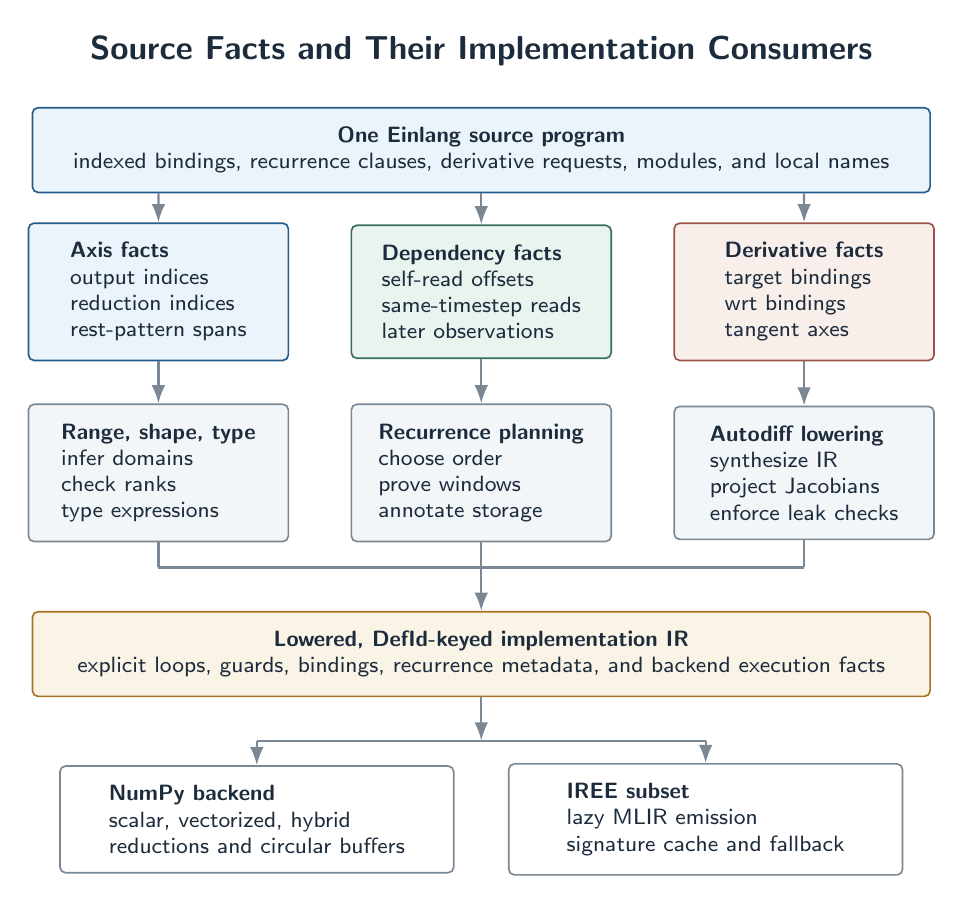
\begin{tikzpicture}[
  font=\sffamily\footnotesize,
  >=Latex,
  title/.style={font=\sffamily\bfseries\large,text=figInk,align=center},
  box/.style={draw=figLine,line width=0.6pt,rounded corners=2pt,fill=white,align=left,inner sep=7pt,text=figInk},
  fact/.style={box,minimum width=3.3cm,minimum height=1.25cm},
  consumer/.style={box,minimum width=3.3cm,minimum height=1.25cm,fill=figSlateBg},
  spine/.style={box,minimum width=11.4cm,minimum height=1.0cm,align=center},
  backend/.style={box,minimum width=5.0cm,minimum height=1.1cm,fill=white},
  arrow/.style={->,line width=0.8pt,draw=figLine},
  bus/.style={line width=0.8pt,draw=figLine}
]

\node[title] (title) at (0,0) {Source Facts and Their Implementation Consumers};

\node[spine,fill=figBlueBg,draw=figBlue] (source) at (0,-1.25) {
  \textbf{One Einlang source program}\\
  indexed bindings, recurrence clauses, derivative requests, modules, and local names
};

\node[fact,fill=figBlueBg,draw=figBlue] (axes) at (-4.1,-3.05) {
  \textbf{Axis facts}\\
  output indices\\
  reduction indices\\
  rest-pattern spans
};
\node[fact,fill=figGreenBg,draw=figGreen] (deps) at (0,-3.05) {
  \textbf{Dependency facts}\\
  self-read offsets\\
  same-timestep reads\\
  later observations
};
\node[fact,fill=figRoseBg,draw=figRose] (diffs) at (4.1,-3.05) {
  \textbf{Derivative facts}\\
  target bindings\\
  wrt bindings\\
  tangent axes
};

\node[consumer] (shape) at (-4.1,-5.35) {
  \textbf{Range, shape, type}\\
  infer domains\\
  check ranks\\
  type expressions
};
\node[consumer] (storage) at (0,-5.35) {
  \textbf{Recurrence planning}\\
  choose order\\
  prove windows\\
  annotate storage
};
\node[consumer] (ad) at (4.1,-5.35) {
  \textbf{Autodiff lowering}\\
  synthesize IR\\
  project Jacobians\\
  enforce leak checks
};

\node[spine,fill=figGoldBg,draw=figGold] (lowered) at (0,-7.65) {
  \textbf{Lowered, DefId-keyed implementation IR}\\
  explicit loops, guards, bindings, recurrence metadata, and backend execution facts
};

\node[backend] (numpy) at (-2.85,-9.75) {
  \textbf{NumPy backend}\\
  scalar, vectorized, hybrid\\
  reductions and circular buffers
};
\node[backend] (iree) at (2.85,-9.75) {
  \textbf{IREE subset}\\
  lazy MLIR emission\\
  signature cache and fallback
};

\draw[arrow] ([xshift=-4.1cm]source.south) -- (axes.north);
\draw[arrow] (source.south) -- (deps.north);
\draw[arrow] ([xshift=4.1cm]source.south) -- (diffs.north);

\draw[arrow] (axes.south) -- (shape.north);
\draw[arrow] (deps.south) -- (storage.north);
\draw[arrow] (diffs.south) -- (ad.north);

\coordinate (lowerbus) at (0,-6.55);
\draw[bus] (-4.1,-6.55) -- (4.1,-6.55);
\draw[bus] (shape.south) -- (-4.1,-6.55);
\draw[bus] (storage.south) -- (0,-6.55);
\draw[bus] (ad.south) -- (4.1,-6.55);
\draw[arrow] (lowerbus) -- (lowered.north);

\coordinate (backendbus) at (0,-8.75);
\draw[arrow] (lowered.south) -- (backendbus);
\draw[bus] (-2.85,-8.75) -- (2.85,-8.75);
\draw[arrow] (-2.85,-8.75) -- (numpy.north);
\draw[arrow] (2.85,-8.75) -- (iree.north);

\end{tikzpicture}
}
\caption{Thesis-specific implementation view: source facts are preserved until
the compiler pass that consumes them, then carried into lowered backend-facing
IR.}
\label{fig:fragmentation}
\end{figure}

\chapter{Language Design}

The language design is intentionally small at the surface. A scalar binding
names a value; an indexed binding builds a tensor point by point; a reduction
introduces a local index; a recurrence defines a binding through base and
recurrent clauses; and a derivative request asks for the sensitivity of one
named value with respect to another.

\begin{lstlisting}[style=einlang]
let C[i, j] = sum[k](A[i, k] * B[k, j]);
let x[0] = x0;
let x[t in 1..T] = step(x[t - 1], u[t]);
let dx0 = @x[T - 1] / @x0;
\end{lstlisting}

The matrix multiplication line exposes output axes \texttt{i} and \texttt{j}
and reduction axis \texttt{k}. The recurrence exposes the self-read offset
\texttt{t - 1}. The derivative request names the target and parameter at the
point where the sensitivity is needed.

The example is intentionally small, but it shows the thesis boundary. The
compiler does not receive an opaque tensor call followed by a host loop followed
by an AD transform; it receives three source constructs in one binding
environment. That means the name resolver, range analysis, recurrence analysis,
and autodiff passes can agree on the same DefIds. The programmer still writes
mathematical notation, while the implementation keeps enough structure to make
compile-time checks and lowering choices before execution.

\section{Indexed Definitions}

An indexed binding defines a tensor over an index environment. Explicit ranges
such as \texttt{i in 0..M} attach domains directly to variables. When ranges are
omitted, shaped tensor reads can provide candidate domains: a read of
\texttt{A[i,k]} constrains \texttt{i} to the first axis of \texttt{A} and
\texttt{k} to the second. Reduction indices follow the same rule inside the
reduction body.

\begin{lstlisting}[style=einlang]
let Y[n in 0..N, o in 0..OC, i in 0..OH, j in 0..OW] =
    sum[c in 0..IC, r in 0..KH, s in 0..KW](
        X[n, c, i + r, j + s] * W[o, c, r, s]);
\end{lstlisting}

This direct convolution keeps surviving axes, reduction axes, and affine input
offsets in one source expression. An \texttt{einsum}-plus-patches encoding can
run the same computation, but it splits the sliding-window construction from the
contraction. \einlang{} keeps both facts in one binding.

The analysis value is the combination, not only the notation. The output axes
\texttt{n}, \texttt{o}, \texttt{i}, and \texttt{j} define the produced tensor,
while the reduction axes \texttt{c}, \texttt{r}, and \texttt{s} define the
contracted kernel domain. The affine offsets \texttt{i + r} and \texttt{j + s}
also remain visible to bounds checking and lowering. A backend may still choose
to run this as patches, scalar loops, or a vectorized contraction, but that is a
later execution decision rather than the source-level representation.

\begin{center}
\centering
\begin{minipage}[t]{0.48\linewidth}
\textbf{Einlang: named axes in IR}
\begin{lstlisting}[style=einlang,basicstyle=\ttfamily\footnotesize]
let C[i, j] =
    sum[k](A[i, k] * B[k, j]);
\end{lstlisting}
\end{minipage}
\hfill
\begin{minipage}[t]{0.48\linewidth}
\textbf{NumPy: string mini-language}
\begin{lstlisting}[style=pythoncode,basicstyle=\ttfamily\footnotesize]
C = np.einsum("ik,kj->ij", A, B)
\end{lstlisting}
\end{minipage}

\vspace{0.45\baselineskip}
\begin{minipage}[t]{0.48\linewidth}
\textbf{TVM: tensor expression}
\begin{lstlisting}[style=pythoncode,basicstyle=\ttfamily\footnotesize]
k = te.reduce_axis((0, K), "k")
C = te.compute((M, N),
    lambda i, j: te.sum(
        A[i, k] * B[k, j], axis=k))
\end{lstlisting}
\end{minipage}
\hfill
\begin{minipage}[t]{0.48\linewidth}
\textbf{Halide: update definition}
\begin{lstlisting}[style=pythoncode,basicstyle=\ttfamily\footnotesize]
Var i, j;
RDom k(0, K);
Func C;
C(i, j) += A(i, k) * B(k, j);
\end{lstlisting}
\end{minipage}

\captionsetup{type=figure,hypcap=false}
\caption{Thesis-adapted comparison of indexed reduction interfaces. The reused
paper example is copied into the thesis figure set and retuned around compiler
facts rather than presentation brevity.}
\label{fig:thesis-indexed-reduction-interfaces}
\end{center}

Figure~\ref{fig:thesis-indexed-reduction-interfaces} should be read as a
compiler-boundary comparison. NumPy places the contraction structure in a
string, which is compact but separated from ordinary name resolution. TVM and
Halide expose structured tensor expressions, but they are embedded in host-side
scheduling systems. The \einlang{} form keeps the same source binding, the same
index variables, and the same diagnostics context available to later passes.
That is why the thesis treats indexed notation as an implementation contract
rather than as surface sugar.

\subsection{Index Domains and Where Clauses}

Index domains are intentionally attached to index positions rather than hidden
inside a separate loop statement. This matters for diagnostics and lowering. A
range such as \texttt{i in 0..M} is in scope for the indexed body, and a
reduction range such as \texttt{k in 0..K} is in scope only for the reduction
body. Predicate-style \texttt{where} clauses refine a domain, while iteration
ranges in \texttt{where} clauses are rejected by validation because they obscure
which source construct owns the index.

\begin{lstlisting}[style=einlang]
let even_square[i in 0..N] = i * i where i % 2 == 0;
let total = sum[k in 0..N](even_square[k]);
\end{lstlisting}

The implementation uses this discipline in range analysis: every index variable
has a DefId, and all inferred domains are keyed by that DefId. The same spelling
can be reused in separate indexed bindings without aliasing compiler state.

The two-line example demonstrates both parts of the rule. The first binding
creates a tensor only over even points in \texttt{0..N}; the second reduction
then consumes that tensor through an ordinary loop variable. Because the
\texttt{where} predicate is not itself a new iteration domain, the compiler can
classify it as a guard. That distinction matters later: guards become lowered
conditions, while ranges become loop bounds. Collapsing the two would make it
harder to explain diagnostics and harder for the backend to choose a correct
execution strategy.

\section{Declarative Recurrence}

A recurrent binding may have multiple clauses. Base clauses define boundary
points; recurrent clauses define the remaining domain and may read other points
of the same binding.

\begin{lstlisting}[style=einlang]
let H[0, j in 0..N] = top[j];
let H[i in 0..M, 0] = left[i];
let H[i in 1..M, j in 1..N] =
    mix(H[i - 1, j], H[i, j - 1], input[i, j]);
\end{lstlisting}

The source contract is dependency, not schedule. The compiler must evaluate each
point after the points it reads, but the source program does not have to pick a
loop nest, carry tuple, row buffer, or full materialization policy up front.

This example is a two-dimensional dependency relation. The interior clause
reads one point above and one point to the left, so a legal traversal must
respect both predecessor directions. The source does not say whether rows,
columns, tiles, or a full materialized grid should be used; it states the
relation that any such schedule must satisfy. The implementation can therefore
derive recurrence dimensions and storage metadata from reads of the same DefId,
instead of attempting to reverse-engineer a relation from already-written host
control flow.

\begin{center}
\centering
\begin{minipage}[t]{0.48\linewidth}
\textbf{Einlang: dependency relation}
\begin{lstlisting}[style=einlang,basicstyle=\ttfamily\footnotesize]
let y[0] = init;
let y[t in 1..T] =
    step(y[t - 1], x[t]);
let out = y[T - 1];
\end{lstlisting}
\end{minipage}
\hfill
\begin{minipage}[t]{0.48\linewidth}
\textbf{JAX: carry contract}
\begin{lstlisting}[style=pythoncode,basicstyle=\ttfamily\footnotesize]
def body(carry, x_t):
    y = step(carry, x_t)
    return y, y
out, ys = jax.lax.scan(
    body, init, x[1:])
\end{lstlisting}
\end{minipage}

\vspace{0.45\baselineskip}
\begin{minipage}[t]{0.48\linewidth}
\textbf{PyTorch: host storage}
\begin{lstlisting}[style=pythoncode,basicstyle=\ttfamily\footnotesize]
ys = [init]
for x_t in x[1:]:
    ys.append(step(ys[-1], x_t))
out = ys[-1]
\end{lstlisting}
\end{minipage}
\hfill
\begin{minipage}[t]{0.48\linewidth}
\textbf{Compiler-visible fact}
\begin{lstlisting}[style=pythoncode,basicstyle=\ttfamily\footnotesize]
self_reads = {t: t - 1}
order = topological_order(self_reads)
storage = bounded_window(self_reads)
\end{lstlisting}
\end{minipage}

\captionsetup{type=figure,hypcap=false}
\caption{Thesis-adapted comparison of recurrence interfaces. The thesis copy
emphasizes which scheduling and storage decisions are source obligations in
neighboring systems and which are compiler obligations in \einlang{}.}
\label{fig:thesis-recurrence-interfaces}
\end{center}

Figure~\ref{fig:thesis-recurrence-interfaces} highlights the delayed
commitment. JAX asks the user to choose a carry boundary and stacked output
shape before the compiler sees later observations. A PyTorch loop makes storage
an ordinary host-language list decision. In \einlang{}, the self-read offset is
the source fact; traversal order and finite-window storage are compiler
obligations. This difference is small in a one-step recurrence, but it becomes
important when later code observes only a suffix, a final value, or an
intermediate derivative.

\subsection{Boundary Clauses}

Base and recurrent clauses share one binding name. The grouping pass therefore
sees the following as one recurrent definition rather than as unrelated
assignments:

\begin{lstlisting}[style=einlang]
let fib[0] = 0;
let fib[1] = 1;
let fib[n in 2..N] = fib[n - 1] + fib[n - 2];
\end{lstlisting}

This source form is small, but it carries three compiler facts: the covered
boundary points, the recurrent domain, and the static self-read offsets. Those
facts are consumed later by lowering, recurrence-order analysis, and storage
planning.

The base clauses are not special cases outside the binding. They are part of
the same grouped definition as the recurrent clause, which lets the compiler
check that the values read by \texttt{fib[n - 1]} and \texttt{fib[n - 2]} are
available when the recurrent body runs. The same grouping also prevents the
runtime from treating the three statements as independent outputs. The
important analysis point is that boundary coverage and recurrence dependency
are represented together, so storage inference can distinguish required
history from values that only initialize the sequence.

\section{Local Derivative Requests}

Derivative requests are expressions over named source bindings:

\begin{lstlisting}[style=einlang]
let loss = sum[i]((pred[i] - target[i]) * (pred[i] - target[i]));
let dloss_dW = @loss / @W;
\end{lstlisting}

The target and parameter names determine the derivative shape. Because the
request is an expression, it can appear near the computation it differentiates,
including near intermediate or recurrent values. This is narrower than a full
host-language AD system, but it gives the source language a simple and local
differentiation interface.

The quotient form is restricted to named source bindings because this makes the
compiler's dependency query precise. A derivative of an anonymous inline
subexpression would force the compiler to invent a hidden binding and decide its
scope. \einlang{} instead asks the programmer to name the value, which also
improves diagnostics and reuse.

The two-line derivative example is deliberately source-local. The user names
the loss once, then asks for the sensitivity with respect to \texttt{W} where
the result is needed. The compiler can use the DefId of \texttt{loss} as the
target and the DefId of \texttt{W} as the parameter, so the request is a
structured dependency query rather than a string or callback. This is also why
anonymous derivatives are not the core interface: naming the target gives the
implementation a stable node to analyze, cache, lower, and report in
diagnostics.

\begin{center}
\centering
\begin{minipage}[t]{0.48\linewidth}
\textbf{Einlang: shaped source expression}
\begin{lstlisting}[style=einlang,basicstyle=\ttfamily\footnotesize]
let local[t, j] =
    @h[t, j] / @theta[j];
\end{lstlisting}
\end{minipage}
\hfill
\begin{minipage}[t]{0.48\linewidth}
\textbf{JAX: package selected value}
\begin{lstlisting}[style=pythoncode,basicstyle=\ttfamily\footnotesize]
local = jax.grad(
    lambda th: run(th)[t, j]
)(theta)[j]
\end{lstlisting}
\end{minipage}

\vspace{0.45\baselineskip}
\begin{minipage}[t]{0.48\linewidth}
\textbf{Julia/Zygote: closure boundary}
\begin{lstlisting}[style=pythoncode,basicstyle=\ttfamily\footnotesize]
using Zygote
local = gradient(
    th -> run(th)[t, j], theta
)[1][j]
\end{lstlisting}
\end{minipage}
\hfill
\begin{minipage}[t]{0.48\linewidth}
\textbf{PyTorch: graph-state query}
\begin{lstlisting}[style=pythoncode,basicstyle=\ttfamily\footnotesize]
h = run(theta)
theta.grad = None
h[t, j].backward()
local = theta.grad[j]
\end{lstlisting}
\end{minipage}

\captionsetup{type=figure,hypcap=false}
\caption{Thesis-adapted comparison of local derivative interfaces. The thesis
copy keeps the paper's motivating query but retunes the labels around the
implementation boundary that the autodiff passes consume.}
\label{fig:thesis-local-derivative-interfaces}
\end{center}

Figure~\ref{fig:thesis-local-derivative-interfaces} compares where the
derivative boundary appears. JAX and Zygote package the selected value behind a
function-like object; PyTorch exposes the query through graph state and a
gradient buffer. \einlang{} instead makes the sensitivity an expression whose
shape follows from the target and parameter. The implementation burden is
higher because the compiler must lower the shaped request, but the source
benefit is that intermediate and recurrent sensitivities stay in the same
indexed language as the values they describe.

\section{Types and Values}

The executed implementation supports primitive scalars, rectangular arrays,
jagged arrays for non-Einstein data, tuples, function values, and differential
types used during the autodiff phase. Rectangular arrays are the tensor type
that participates in indexed notation. A type can specify concrete dimensions,
unknown dimensions, or dynamic rank:

\begin{lstlisting}[style=einlang]
let x: f32 = 1.0;
let v: [f32] = [1.0, 2.0, 3.0];
let m: [f32; 2, 3] = [[1.0, 2.0, 3.0], [4.0, 5.0, 6.0]];
let dyn: [f32; *] = load_npy("weights.npy");
\end{lstlisting}

Shape is not only a type annotation. The compiler separately computes
expression-level shape facts from literals, indexed definitions, reductions,
and calls. This separation lets the type system track precision and rank while
shape analysis tracks the concrete dimensions needed for indexing and lowering.

The example distinguishes four levels of precision. A scalar has a primitive
type only; a vector fixes rank but may leave length dynamic; a rectangular
literal can expose concrete dimensions; and a loaded array may have dynamic
rank. The compiler keeps these cases separate so that a function can be type
compatible even when a later range or lowering pass still needs a concrete
shape fact. In other words, type checking decides whether an expression is a
tensor-like value of the right element kind, while shape analysis decides which
indices and loops are legal for that value.

\section{Functions, Blocks, and Modules}

Functions are expressions with parameters, optional type annotations, and an
implicit return value equal to the final block expression. Functions can be
called before their textual definition after name resolution has hoisted item
bindings. Modules are file-backed units resolved through \texttt{use} and
\texttt{mod} declarations. Public functions and public re-exports make the
standard library usable as ordinary \einlang{} code rather than as a bag of
compiler intrinsics.

\begin{lstlisting}[style=einlang]
use std::math::basic::sqrt;

fn norm2(x, y) {
    sqrt(x * x + y * y)
}

let r = norm2(3.0, 4.0);
\end{lstlisting}

This snippet shows the ordinary-language machinery that the tensor features
depend on. The \texttt{use} statement must resolve through the module system
before the function call can be typed, and the function body must be hoisted so
the call site can refer to a stable DefId. The final expression of the block is
the return value, which keeps functions lightweight enough to use in indexed
bodies. Without this module and function layer, the tensor core would collapse
into a set of builtins rather than a language with reusable source libraries.

The example also shows why ordinary expression features are part of the
implementation story rather than background convenience. A standard-library
function such as \texttt{sqrt} has to be imported, assigned a DefId, checked as
a callable value, and executed through the same backend path as user functions.
The final-expression return rule lets helper functions remain small enough to
appear naturally inside tensor bodies, while the module system lets those
helpers live outside the compiler. This is what keeps tensor notation from
becoming a closed DSL with only hard-coded operations.

\section{General Language Surface}

The implementation supports more than the tensor core. The grammar includes
function definitions, public functions, \texttt{@fn} differential rules, typed
parameters and returns, immutable \texttt{let} and \texttt{const} declarations,
tuple destructuring, blocks as expressions, \texttt{if}, \texttt{match},
patterns, arrays, tuples, member access, pipeline expressions, casts,
interpolated strings, module paths, \texttt{use} statements, inline modules,
struct and enum syntax, and where clauses. Some parsed surface forms are
implemented as current language features, while some remain parsed but not yet
fully supported by the backend. The thesis focuses on the non-trivial executed
path: tensor definitions, functions, modules, typing, recurrences, autodiff,
standard-library calls, and examples.

\section{Composition}

The constructs are designed to be orthogonal. An indexed definition can feed a
recurrence; a recurrence can feed an indexed reduction; a derivative request can
target a final scalar or an intermediate tensor. The language benefit is stable
notation. The compiler benefit is that the same IR can carry axes, domains,
dependency offsets, and derivative targets until the pass that consumes each
fact has run.

\begin{lstlisting}[style=einlang]
let score[t] = sum[d](x[t, d] * w[d]);
let prefix[0] = score[0];
let prefix[t in 1..T] = prefix[t - 1] + score[t];
let dw = @prefix[T - 1] / @w;
\end{lstlisting}

The same source region contains a contraction, a recurrent binding, and a local
derivative request. In a host framework this would typically become an array
operation, a loop or scan, and a separate AD call. In \einlang{}, the compiler
sees the named axes, the recurrent dependency, and the derivative target before
any of them are lowered to backend operations.

Composition is the strongest reason to keep the constructs in one language.
The \texttt{score} binding exposes an indexed contraction, \texttt{prefix}
turns that value into a recurrent sequence, and \texttt{dw} asks for a
derivative of the final recurrent value. Each line consumes facts produced by
earlier lines without changing notation families. The compiler can therefore
thread range facts, recurrence offsets, and autodiff dependencies through one
IR instead of coordinating several external APIs. This is the source-level
version of the implementation thesis: smart passes become possible because the
program has not hidden its structure too early.

\chapter{Frontend, Names, and Modules}

The front end turns source text into a source-located AST and then into a
DefId-resolved IR. This part of the implementation is non-trivial because
\einlang{} is not only an expression language: it has modules, imports,
function hoisting, index scopes, named rest patterns, and local derivative
syntax.

\section{Parsing and AST Construction}

The parser in \pathcode{src/einlang/frontend/parser.py} wraps a shared Lark LALR
parser loaded from \pathcode{src/einlang/frontend/grammar.lark}. The shared
parser is keyed by cache path so repeated compilations do not rebuild grammar
tables. Disk parser caches are disabled by default, but the code can use an
explicit cache path when configured. The parser propagates source positions and
converts Lark errors into \einlang{} parse errors with source locations.

AST construction is handled by frontend transformers under
\pathcode{src/einlang/frontend/transformers}. The transformer layer is split by
concern: base expression and statement construction, function-specific logic,
literals, and string interpolation. This split matters because later compiler
passes assume that syntax has already been normalized into the AST node classes
in \pathcode{src/einlang/shared/nodes.py}.

The transformer is not just a mechanical parse-tree adapter. It constructs
source spans, normalizes equivalent surface forms, attaches structured nodes for
patterns and type annotations, and records interpolation pieces so the backend
can later evaluate a string expression without reparsing source text. Lark
therefore supplies the parsing engine, but \einlang{} still owns the language
grammar and the AST shape consumed by later compiler phases.

\section{Grammar Coverage}

The grammar contains the executed tensor subset and the broader language shape.
It parses:

\begin{itemize}
\item declarations: \texttt{fn}, \texttt{pub fn}, \texttt{@fn},
\texttt{let}, \texttt{const}, and indexed Einstein declarations;
\item expressions: arithmetic, logic, ranges, casts, calls, member access,
array access, array literals, comprehensions, tuples, blocks, \texttt{if},
\texttt{match}, lambdas, pipelines, and \texttt{try};
\item tensor syntax: rectangular access, reductions, explicit index ranges,
literal indices, and named rest indices such as \texttt{..batch};
\item modules: \texttt{use}, wildcard imports, list imports, aliases,
\texttt{mod}, public modules, and inline modules;
\item types: primitive, rectangular, jagged, tuple, function, generic, and
named types.
\end{itemize}

The important implementation choice is that tensor notation is not parsed as a
separate mini-language. It participates in the same expression grammar as the
rest of the source program.

\section{DefId-Based Identity}

Names become semantic identifiers during name resolution. The DefId system in
\pathcode{src/einlang/shared/defid.py} follows the rustc pattern: a definition
identifier is a pair \texttt{(krate, index)}. User code uses crate 0, and
builtins use a separate builtin crate with fixed DefIds for values such as
\texttt{print}, \texttt{assert}, \texttt{len}, \texttt{shape}, \texttt{sum},
\texttt{max}, and \texttt{min}.

This design removes ambiguity from later stages. Once name resolution has run,
runtime lookup and compiler analyses use DefIds rather than strings. Strings
remain for diagnostics and debugging, but they do not decide identity. This is
especially important for index variables and local variables because the same
spelling may appear in different scopes.

\section{Name Resolution and Scope}

The name-resolution pass in \pathcode{src/einlang/passes/name_resolution.py}
allocates DefIds, resolves use sites, handles builtins, assigns DefIds to
parameters and locals, and wires functions and modules into the compilation
context. Function differential rules are first merged into ordinary functions by
\pathcode{src/einlang/passes/merge_diff_rules.py}, so the compiler sees one
function definition with attached differential behavior instead of two
unrelated definitions.

The scope system in \pathcode{src/einlang/shared/scope.py} tracks scope kind and
binding type. Local variable DefIds are allocated without inserting them into
the global symbol table; item-like definitions such as functions, constants,
modules, and builtins are registered in the resolver tables. That separation is
what lets local shadowing work without corrupting module-level lookup.

\subsection{Resolution Algorithm}

The resolver is a two-level identity algorithm. Item-like names are installed in
module-level maps, while local names are installed only in lexical scopes. Every
use site is rewritten from a string name to a DefId before later passes run.
The key invariant is simple: after resolution, semantic equality is DefId
equality.

\begin{lstlisting}[style=pythoncode,caption={DefId-based name resolution.}]
resolve_program(ast, tcx):
    group_consecutive_einstein_declarations(ast)
    install_fixed_builtins(tcx.resolver)
    load_and_link_imported_modules(ast, tcx.module_loader, tcx.symbol_linker)

    # Hoist item identities before resolving bodies.
    for item in ast.top_level_items:
        if item is function or constant or module:
            did = resolver.allocate_for_item(item.module_path, item.name)
            item.defid = did
            resolver.register(did, item)
            current_module.define(item.name, Binding(did, ITEM))

    for item in ast.top_level_items:
        resolve_item_body(item)

resolve_item_body(item):
    with scope(kind=FUNCTION_OR_MODULE):
        for parameter in item.parameters:
            did = resolver.allocate_for_local()
            parameter.defid = did
            scope.define(parameter.name, Binding(did, PARAMETER))
        resolve_expr(item.body)

resolve_expr(expr):
    case local binding:
        resolve_expr(expr.value)
        did = resolver.allocate_for_local()
        expr.defid = did
        scope.define(expr.name, Binding(did, LOCAL))
    case identifier:
        binding = scope.lookup(expr.name) or module_lookup(expr.name)
        expr.defid = binding.defid
    case indexed clause:
        with scope(kind=INDEX):
            allocate DefIds for output indices and where-bindings
            resolve body and guard expressions in that scope
    case nested block:
        with scope(kind=BLOCK):
            resolve statements in source order
\end{lstlisting}

This algorithm explains why shadowing is safe. A local \texttt{i} in one
Einstein clause and another local \texttt{i} in a different clause may share a
printed name, but their DefIds differ. Range, shape, type, lowering, and
runtime lookup therefore do not need to guess which \texttt{i} a later node
means.

The listing is longer than a conventional symbol-table sketch because the
resolver is also the first pass that makes tensor syntax semantically precise.
Top-level hoisting gives functions and constants stable identities before their
bodies are visited, which permits forward references and module-level cycles to
be diagnosed at the right boundary. Local allocation is intentionally separate:
parameters, block locals, and index variables live in lexical scopes and do not
pollute the module table. This is the property that allows a tensor clause to
introduce \texttt{i} without changing the meaning of a neighboring clause.

The indexed-clause case is especially important. Output indices and
where-bound variables are allocated in an index scope before the body is
resolved, so every rectangular access and reduction body can point at the
precise DefId it uses. Later passes never need to inspect textual names to
recover that relationship. If a diagnostic still wants to print the spelling
\texttt{i}, it can do so as presentation; the compiler's semantic decisions are
already made from DefIds. That split between user-facing names and compiler
identity is one of the main reasons the rest of the implementation can remain
modular.

The ordering of the traversal is also part of the algorithm's correctness.
Hoisting items before resolving bodies means that a call can refer to a
function that appears later in the file, while local bindings remain
source-ordered so a block cannot accidentally use a value before it is
introduced. The resolver therefore uses two different temporal models: an
item-level model for modules and functions, and a statement-level model for
locals. This split is small in code, but it is what lets \einlang{} support both
ordinary function libraries and expression-like blocks without a second
resolution mechanism.

The failure modes are designed to remain source-facing. An unresolved
identifier is reported at the use site, not at a later backend lookup; an
attempt to bind an index in the wrong scope is rejected while the compiler still
knows which clause introduced it; and an imported name conflict is reported
against the relevant \texttt{use} declaration. The later compiler can then
treat missing DefIds as internal bugs rather than user errors. This is an
important thesis point: the resolver turns textual ambiguity into either a
stable identity or an early diagnostic, and every smart pass depends on that
binary outcome.

\textit{Concrete example.} In a program containing \texttt{fn norm(x) \{ let
x = x * x; x \}} and a separate indexed binding \texttt{let y[i] = x[i];}, the
printed name \texttt{x} names three different things: the function parameter,
the local square, and the top-level tensor read by \texttt{y}. Resolution gives
each binding its own DefId before type or shape analysis runs. The local
\texttt{x} shadows the parameter only inside the function body, while the
\texttt{x[i]} read in the indexed binding still points to the top-level tensor.
This is the concrete reason later passes do not carry name-disambiguation code:
they see only DefIds and scopes that have already been checked.

\begin{table}[htbp]
\centering
\caption{Representative DefId ownership rules.}
\label{tab:defid-rules}
\renewcommand{\arraystretch}{1.08}
\begin{tabular}{@{}L{0.26\textwidth}L{0.62\textwidth}@{}}
\toprule
Definition kind & Resolution behavior \\
\midrule
Builtins & Allocated in a fixed builtin crate so runtime and compiler can agree on names such as \texttt{print}, \texttt{shape}, and \texttt{\_\_basis\_tensor}. \\
Functions and constants & Registered in the module symbol table and resolver registry. They can be imported, re-exported, and looked up by module path. \\
Parameters and locals & Allocated as local DefIds and attached to definitions and use sites, but not inserted into the global symbol table. \\
Index variables & Allocated as local DefIds so repeated spellings such as \texttt{i} in different indexed bindings remain distinct. \\
Generated indices & Allocated by the resolver when rest-pattern or lowering passes need compiler-created loop variables. \\
\bottomrule
\end{tabular}
\end{table}

\section{Module Loading}

\einlang{} modules are file based. The module system under
\pathcode{src/einlang/analysis/module_system} resolves module paths, loads
source, parses module ASTs, detects circular imports, processes submodule
declarations, and handles exported symbols. The path resolver follows
Rust-inspired rules:

\begin{itemize}
\item \texttt{std::math} resolves into the bundled standard-library tree;
\item \texttt{crate::x}, \texttt{self::x}, and \texttt{super::x} are handled as
structured module paths;
\item project-local modules resolve relative to the crate root;
\item \texttt{python::...} is a virtual path for Python module integration.
\end{itemize}

Module loading is performance-sensitive because standard-library modules are
used repeatedly. The loader caches file contents and parsed ASTs in process, and
can optionally use a disk parse cache when \texttt{EINLANG\_CACHE\_DIR} is set.
Callers receive fresh AST copies because later compiler passes mutate node
metadata.

The loader also supports source overlays. Tests and embedding callers can supply
in-memory module sources keyed by module path, avoiding filesystem reads while
still exercising the same module and name-resolution code as normal programs.

\subsection{Module Loading Algorithm}

Module loading is deliberately written as a cache-and-copy algorithm. The
cached object is parsed syntax; the returned object is a fresh copy that later
passes may annotate or mutate.

\begin{lstlisting}[style=pythoncode,caption={Source overlay and module-cache resolution.}]
load_module(path, requester):
    normalized = path_resolver.resolve(path, requester)
    if normalized in active_import_stack:
        report circular import

    if normalized in source_overlays:
        source = source_overlays[normalized]
        cache_key = ("overlay", normalized, hash(source))
    else:
        file_path = path_resolver.to_file(normalized)
        source = read_file_cached(file_path)
        cache_key = ("file", file_path, mtime_or_content_key)

    if cache_key not in parsed_ast_cache:
        parsed_ast_cache[cache_key] = parse_source(source)

    ast = deep_copy(parsed_ast_cache[cache_key])
    active_import_stack.push(normalized)
    process_submodules_and_use_statements(ast)
    active_import_stack.pop()
    return ast
\end{lstlisting}

The overlay branch is important for tests and embedding: it makes synthetic
modules go through the same import, symbol-linking, and resolution machinery as
files on disk. The deep-copy step is equally important because downstream IR
and AST passes attach DefIds, types, shapes, ranges, and lowering facts.

The cache stores parsed syntax rather than analyzed syntax. That choice avoids
sharing mutable compiler annotations between compilations, which would be a
subtle source of stale DefIds, stale shape facts, or stale diagnostics. A cache
hit therefore saves parsing work but still returns a tree that the caller can
own. This is a conservative design: it gives repeated stdlib imports and tests
the performance benefit of caching without turning later passes into
copy-on-write clients of a global AST.

The active import stack is the other non-trivial part of the algorithm. Module
loading is recursive because a module may declare submodules or import other
paths while it is being processed. Recording the normalized path before
descending lets the loader report circular imports as source errors rather than
recursing indefinitely. The same normalized path also lets source overlays and
filesystem modules share the symbol-linking path, which keeps test fixtures and
real projects behaviorally aligned.

The cache key design prevents a subtle class of bugs. Overlay modules are keyed
by content hash because two tests may reuse the same logical module path with
different in-memory source. Filesystem modules are keyed by a file-derived
freshness value, so editing a standard-library file can invalidate the cached
parse tree. In both cases the cached artifact is syntax only. DefIds, types,
shapes, and module exports are deliberately recomputed because they depend on
the compilation context that requested the module.

The algorithm also makes module loading compositional. A module can import a
submodule, that submodule can import a sibling, and all of those paths collapse
to normalized module identities before caching and cycle detection run. This is
why the circular-import stack stores normalized paths rather than raw source
strings. Without normalization, \texttt{self::x}, \texttt{crate::m::x}, and a
relative filesystem spelling could look different while naming the same module.
The loader's job is to collapse those spellings before the resolver assigns
semantic identities to exported items.

\textit{Concrete example.} A source file that says \texttt{use
std::math::basic::sqrt;} first resolves the path to the bundled stdlib module,
then parses or reuses the cached AST for that module, then returns a fresh copy
for this compilation. A test may override the same logical path with a source
overlay defining a tiny fake \texttt{sqrt}; the cache key includes the overlay
contents, so that fake module cannot poison later filesystem loads. In both
cases the resolver receives an ordinary module AST and assigns DefIds to the
exported function in the requesting compilation context.

\section{Imports, Aliases, and Re-exports}

The symbol linker resolves \texttt{use} statements into function mappings and
module aliases. It supports direct imports, wildcard imports, module aliases,
and public re-exports. For example, \texttt{use std::math::basic::sqrt;} maps
the visible name \texttt{sqrt} to the module that exported it, while
\texttt{use std::math as m;} creates an alias used by later module-access
expressions.

This module machinery is not decoration around the core language. The standard
library, examples, and tests depend on it, and the implementation treats stdlib
functions as ordinary \einlang{} code rather than as compiler magic whenever
possible.

\chapter{IR and Compiler Pass Pipeline}

The compiler driver in \pathcode{src/einlang/compiler/driver.py} orchestrates
the implementation. It parses source, constructs the module system, merges
differential rules, resolves names, lowers AST to IR, runs the pass pipeline,
tree-shakes unused code, and returns a compilation result. The runtime receives
IR that has already been annotated with the facts needed by the backend.

\begin{figure}[p]
\centering
\resizebox{\textwidth}{!}{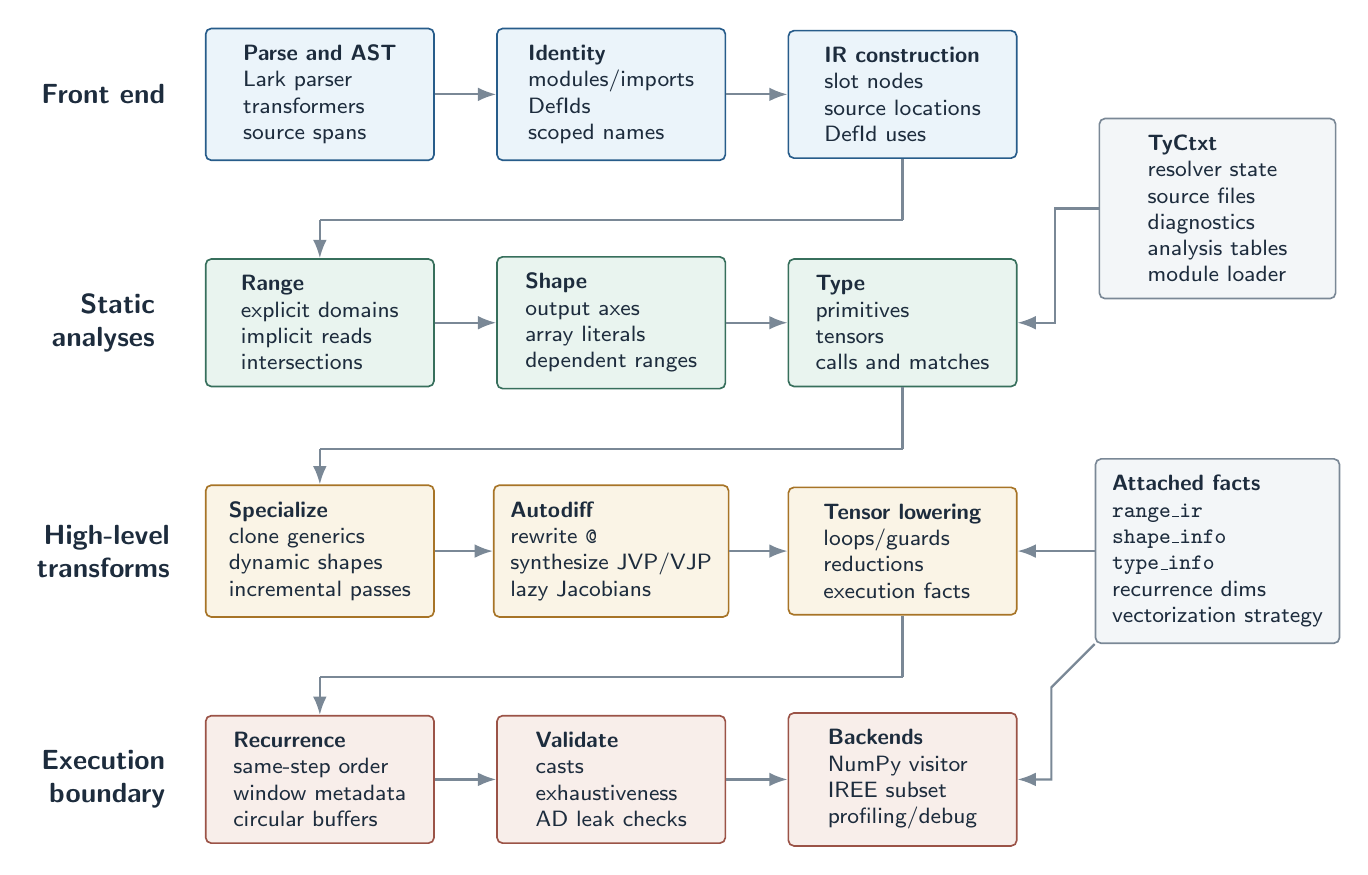
\begin{tikzpicture}[
  font=\sffamily\footnotesize,
  >=Latex,
  stage/.style={draw=figLine,line width=0.6pt,rounded corners=2pt,fill=white,align=left,inner sep=6pt,text=figInk,minimum width=2.9cm,minimum height=1.2cm},
  phase/.style={stage,fill=figBlueBg,draw=figBlue},
  analysis/.style={stage,fill=figGreenBg,draw=figGreen},
  lowering/.style={stage,fill=figGoldBg,draw=figGold},
  runtime/.style={stage,fill=figRoseBg,draw=figRose},
  side/.style={draw=figLine,line width=0.6pt,rounded corners=2pt,fill=figSlateBg,align=left,inner sep=6pt,text=figInk,minimum width=3.0cm},
  arrow/.style={->,line width=0.8pt,draw=figLine},
  bus/.style={line width=0.8pt,draw=figLine},
  rowlabel/.style={font=\sffamily\bfseries,text=figInk,align=right}
]

\node[rowlabel] at (-1.5,0) {Front end};
\node[phase] (parse) at (1.25,0) {
  \textbf{Parse and AST}\\
  Lark parser\\
  transformers\\
  source spans
};
\node[phase] (resolve) at (4.95,0) {
  \textbf{Identity}\\
  modules/imports\\
  DefIds\\
  scoped names
};
\node[phase] (ir) at (8.65,0) {
  \textbf{IR construction}\\
  slot nodes\\
  source locations\\
  DefId uses
};

\node[rowlabel] at (-1.5,-2.9) {Static\\analyses};
\node[analysis] (range) at (1.25,-2.9) {
  \textbf{Range}\\
  explicit domains\\
  implicit reads\\
  intersections
};
\node[analysis] (shape) at (4.95,-2.9) {
  \textbf{Shape}\\
  output axes\\
  array literals\\
  dependent ranges
};
\node[analysis] (type) at (8.65,-2.9) {
  \textbf{Type}\\
  primitives\\
  tensors\\
  calls and matches
};

\node[rowlabel] at (-1.5,-5.8) {High-level\\transforms};
\node[lowering] (mono) at (1.25,-5.8) {
  \textbf{Specialize}\\
  clone generics\\
  dynamic shapes\\
  incremental passes
};
\node[lowering] (ad) at (4.95,-5.8) {
  \textbf{Autodiff}\\
  rewrite \texttt{@}\\
  synthesize JVP/VJP\\
  lazy Jacobians
};
\node[lowering] (ein) at (8.65,-5.8) {
  \textbf{Tensor lowering}\\
  loops/guards\\
  reductions\\
  execution facts
};

\node[rowlabel] at (-1.5,-8.7) {Execution\\boundary};
\node[runtime] (rec) at (1.25,-8.7) {
  \textbf{Recurrence}\\
  same-step order\\
  window metadata\\
  circular buffers
};
\node[runtime] (validate) at (4.95,-8.7) {
  \textbf{Validate}\\
  casts\\
  exhaustiveness\\
  AD leak checks
};
\node[runtime] (backend) at (8.65,-8.7) {
  \textbf{Backends}\\
  NumPy visitor\\
  IREE subset\\
  profiling/debug
};

\node[side] (tcx) at (12.65,-1.45) {
  \textbf{TyCtxt}\\
  resolver state\\
  source files\\
  diagnostics\\
  analysis tables\\
  module loader
};
\node[side] (facts) at (12.65,-5.8) {
  \textbf{Attached facts}\\
  \texttt{range\_ir}\\
  \texttt{shape\_info}\\
  \texttt{type\_info}\\
  recurrence dims\\
  vectorization strategy
};

\draw[arrow] (parse.east) -- (resolve.west);
\draw[arrow] (resolve.east) -- (ir.west);
\coordinate (frontbus) at (8.65,-1.6);
\draw[bus] (ir.south) -- (frontbus);
\draw[bus] (frontbus) -- (1.25,-1.6);
\draw[arrow] (1.25,-1.6) -- (range.north);

\draw[arrow] (range.east) -- (shape.west);
\draw[arrow] (shape.east) -- (type.west);
\coordinate (analysisbus) at (8.65,-4.5);
\draw[bus] (type.south) -- (analysisbus);
\draw[bus] (analysisbus) -- (1.25,-4.5);
\draw[arrow] (1.25,-4.5) -- (mono.north);

\draw[arrow] (mono.east) -- (ad.west);
\draw[arrow] (ad.east) -- (ein.west);
\coordinate (loweringbus) at (8.65,-7.4);
\draw[bus] (ein.south) -- (loweringbus);
\draw[bus] (loweringbus) -- (1.25,-7.4);
\draw[arrow] (1.25,-7.4) -- (rec.north);

\draw[arrow] (rec.east) -- (validate.west);
\draw[arrow] (validate.east) -- (backend.west);

\draw[arrow] (tcx.west) -- ++(-0.55,0) |- (type.east);
\draw[arrow] (facts.west) -- (ein.east);
\draw[arrow] (facts.south west) -- ++(-0.55,-0.55) |- (backend.east);

\end{tikzpicture}
}
\caption{Thesis-specific compiler pipeline: the implementation moves from
source identity through static analyses, high-level transforms, recurrence
metadata, validation, and backend execution.}
\label{fig:pipeline}
\end{figure}

\section{Type Context and Pass Manager}

\pathcode{src/einlang/passes/base.py} defines the shared pass interfaces. The
\texttt{TyCtxt} object is the compiler's single context for resolver state,
source files, diagnostics, analysis results, module-system state, source
overlays, and later pass metadata. This mirrors rustc's discipline: passes
communicate through an explicit context instead of through global state.

Passes derive from \texttt{BasePass}; each exposes a \texttt{run} method that
receives the program and \texttt{TyCtxt}. The \texttt{PassManager} records pass
classes and sorts them by declared dependencies. The driver still owns a few
phase boundaries, notably parsing, name resolution, and AST-to-IR lowering.
Later pipeline steps follow the registered pass order.

\subsection{Pass Scheduling Algorithm}

The pass manager is intentionally small. Each pass declares its dependencies,
and the manager converts that dependency graph into an execution order. The
driver then runs passes over the same mutable IR and shared \texttt{TyCtxt}.

\begin{lstlisting}[style=pythoncode,caption={Dependency-ordered pass execution.}]
run_pass_pipeline(program, tcx, requested_passes):
    order = topological_sort(requested_passes, edge = pass.requires)
    for pass_class in order:
        analysis_before = tcx.analysis_table
        program = pass_class().run(program, tcx)
        assert program is not None
        tcx.mark_pass_complete(pass_class)
        validate_declared_outputs_if_enabled(program, analysis_before, tcx)
    return program

topological_sort(passes):
    temporary = set()
    permanent = set()
    out = []

    visit(pass):
        if pass in permanent:
            return
        if pass in temporary:
            report dependency cycle
        temporary.add(pass)
        for dep in pass.requires:
            visit(resolve_pass(dep))
        temporary.remove(pass)
        permanent.add(pass)
        out.append(pass)

    for pass in passes:
        visit(pass)
    return out
\end{lstlisting}

Specialization is the one place where pass scheduling becomes incremental:
type inference may discover a new specialized function, then invoke the prefix
of the pipeline needed to analyze that new body. The same \texttt{TyCtxt}
holds the shared resolver and specialization registry, so the specialized body
can be inserted back into the main program without losing identity.

The scheduling algorithm is deliberately conservative. A pass can only rely on
facts produced by its declared dependencies, and the driver records completion
after a pass has successfully returned a program. This prevents hidden ordering
contracts such as "shape analysis happens to run before type inference" from
living only in the driver's source order. The cycle check is equally important:
analysis passes often grow by consuming newly attached facts, and a dependency
cycle would otherwise turn into a confusing partial analysis rather than an
explicit compiler configuration error.

The validation hook after each pass is an implementation guardrail. Many passes
mutate IR annotations rather than creating a fresh immutable tree, so a pass can
accidentally leave stale facts behind. Capturing the analysis table before the
pass and validating declared outputs gives tests a way to assert that a pass
produced the metadata it promised. This is the practical substitute for a
heavier typed pass framework: the repository stays small, but the pipeline still
has auditable boundaries.

The algorithm is intentionally a scheduler, not a hidden optimizer. It does not
try to reorder passes based on cost or opportunistic shortcuts; it only respects
declared dependencies. That makes pass behavior easier to explain in the thesis:
range analysis is before shape analysis because shape analysis consumes ranges,
not because a particular driver happened to call it first. When a new pass is
added, the author must state what it depends on, and the topological sort either
places it legally or reports a cycle.

This matters for incremental monomorphization as well. A specialized function
created during type inference is not allowed to skip the facts that ordinary
functions receive. The driver can run the required prefix over the clone because
the pass dependencies define that prefix in reusable terms. The result is a
pipeline that can grow dynamically while preserving the same invariants as the
initial program. The small pseudo-code listing therefore captures a larger
engineering principle: compiler phases are explicit contracts, and generated IR
must satisfy the same contracts as source IR.

\textit{Concrete example.} For \texttt{let C[i,j] =
sum[k](A[i,k]*B[k,j]);}, a requested backend execution cannot run type
inference before range analysis, because type inference depends on the shape
facts derived from \texttt{i}, \texttt{j}, and \texttt{k}. The scheduler places
range analysis before shape analysis, shape analysis before type inference, and
type inference before lowering. If a later generic call creates a specialized
matrix helper during type inference, the same dependency prefix is run on the
clone before it rejoins the program. The example shows why pass order is a data
dependency, not a cosmetic list.

\section{IR Node Design}

The IR in \pathcode{src/einlang/ir/nodes.py} is a slot-based class hierarchy.
Every IR node has a source location. Expression nodes carry optional
\texttt{type\_info} and \texttt{shape\_info}. Identity-bearing nodes such as
bindings, parameters, identifiers, functions, index variables, and rest indices
carry DefIds. The visitor interfaces in \pathcode{src/einlang/ir} and
\pathcode{src/einlang/ir/scoped_visitor.py} let passes recurse through the IR
without hand-writing traversal logic for every use.

\subsection{Mutable Analysis Annotations}

Although \einlang{} source bindings are immutable, the compiler IR is not a
formal immutable SSA graph. IR nodes are slot-based Python objects, and passes
attach or update analysis fields such as \texttt{type\_info},
\texttt{shape\_info}, \texttt{range\_ir}, recurrence overrides, execution-facts
IDs, and lowered forms. This is a pragmatic compiler representation: source
values are single-assignment from the user's point of view, while compiler
metadata evolves as each pass learns more.

There is therefore no mutable-to-SSA conversion pass. The compiler instead uses
DefIds for identity and explicit IR nodes for binding, control flow, tensor
clauses, reductions, and lowered loops. If a future backend needs a CFG-style
SSA representation, that would be a new lowering target rather than a
description of the current IR.

\begin{table}[htbp]
\centering
\caption{Important IR families.}
\label{tab:ir-families}
\renewcommand{\arraystretch}{1.08}
\small
\begin{tabular}{@{}L{0.32\textwidth}L{0.56\textwidth}@{}}
\toprule
IR family & Role \\
\midrule
Expression IR & Literals, identifiers, unary and binary operations, calls, blocks, arrays, tuples, casts, member access, control flow, and builtins. \\
Tensor IR & Rectangular access, reduction expressions, Einstein bindings, Einstein clauses, and lowered tensor nodes. \\
Autodiff IR & Differential, JVP, VJP, and lazy-Jacobian request nodes. \\
Binding IR & Top-level and local bindings, functions, constants, parameters, where clauses, modules, and patterns. \\
Lowered IR & Lowered Einstein, reduction, selection, comprehension, and recurrence nodes. \\
\bottomrule
\end{tabular}
\end{table}

IR serialization in \pathcode{src/einlang/ir/serialization.py} supports
S-expression dumps. The CLI exposes this through \texttt{--dump-ir}, which is
important for debugging pass interactions.

\section{Compiler Pipeline}

The registered pipeline is ordered so that source facts are available before
passes consume them. The important passes are:

\begin{table}[p]
\centering
\caption{Main compiler passes and their responsibilities.}
\label{tab:pass-pipeline}
\renewcommand{\arraystretch}{1.08}
\small
\begin{tabular}{@{}L{0.32\textwidth}L{0.56\textwidth}@{}}
\toprule
Pass & Responsibility \\
\midrule
AST to IR lowering & Convert source AST into IR, preserving source locations, DefIds, declarations, expressions, and tensor syntax. \\
Einstein grouping & Group repeated indexed clauses for the same binding into one high-level Einstein binding. \\
Constraint classifier & Classify where-clause predicates and bindings so later range and lowering passes know which constraints are domains, predicates, or value bindings. \\
Rest preprocessing & Expand named rest patterns such as \texttt{..batch} into concrete generated index variables where possible. \\
Range analysis & Infer index ranges from explicit domains, shaped reads, reductions, comprehensions, and constraints. \\
Shape analysis & Compute shapes for expressions and bindings, including array literals, indexed bindings, reductions, offsets, and conditionals. \\
Type inference & Infer scalar precision, array ranks, function types, tuple types, differential types, and call compatibility. \\
Extremum canonicalization & Turn recognized argmax/argmin selection patterns into explicit selection IR. \\
Pre-autodiff pruning & Prune shape/rank branches before differentiation. \\
Autodiff & Expand source differential forms and collect derivative graph facts while high-level tensor IR is still visible. \\
AD request lowering & Lower JVP/VJP/lazy-Jacobian requests into ordinary IR/runtime requests. \\
AD leak check & Ensure source-level \texttt{@} artifacts do not survive past the autodiff phase. \\
Einstein lowering & Lower indexed tensor definitions and reductions into lowered loop/reduction IR. \\
Recurrence order & Infer recurrence dimensions, same-timestep dependencies, execution order hints, and storage metadata. \\
Lowered execution facts & Attach compiler-owned facts that let the backend choose vectorized, scalar, hybrid, or specialized reduction paths without re-analysis. \\
Validation passes & Validate casts, pipeline types, match exhaustiveness, and IR invariants before execution. \\
\bottomrule
\end{tabular}
\end{table}

\section{Range, Shape, and Type}

Range analysis in \pathcode{src/einlang/passes/range_analysis.py} maintains a
DefId-keyed map from index variables to range IR. It intersects multiple
constraints by taking the maximum of starts and the minimum of ends. It also
uses an implicit range detector to recover ranges from tensor reads. Shape
analysis in \pathcode{src/einlang/passes/shape_analysis.py} uses those ranges to
derive output shapes, check rectangular indexing, handle offset expressions, and
annotate expressions with shape facts. Type inference in
\pathcode{src/einlang/passes/type_inference.py} then assigns primitive,
rectangular, tuple, function, and differential types.

The separation is deliberate. Shapes are not stored inside scalar precision
types; rectangular types can mention rank and optional static dimensions, while
shape analysis carries concrete expression-level shape facts. That split keeps
type compatibility and tensor shape reasoning from collapsing into one
monolithic pass.

\subsection{Analysis Flow}

The three analyses form a dependency chain:

\begin{enumerate}
\item Range analysis discovers domains for index variables from explicit
brackets, reductions, comprehensions, shaped reads, and classified constraints.
\item Shape analysis uses those domains to assign shapes to indexed bindings,
array literals, reductions, calls, and control-flow joins.
\item Type inference uses shape and rank information to check operations,
function calls, casts, literals, tuples, and differential values.
\end{enumerate}

This order is what lets code such as matrix multiplication report an index or
shape problem at compile time rather than failing inside a NumPy call.

\begin{lstlisting}[style=einlang]
let C[i, j] = sum[k](A[i, k] * B[k, j]);
\end{lstlisting}

The compiler must infer that \texttt{i} comes from the first axis of
\texttt{A}, \texttt{j} from the second axis of \texttt{B}, and \texttt{k} from
both the second axis of \texttt{A} and the first axis of \texttt{B}. A mismatch
in those inferred \texttt{k} ranges is a source-level shape error.

This one-line program also explains why the analyses are separate. Range
analysis can discover candidate domains for \texttt{i}, \texttt{j}, and
\texttt{k} without yet deciding the element type of the multiplication. Shape
analysis can then use those ranges to infer the result rank and verify that the
contracted axis is compatible. Type inference finally checks whether the
element operations are legal. If those concerns were fused into one pass, every
diagnostic would have to disentangle domain, shape, and element-type failures
after the fact.

The line also illustrates how source structure affects error locality. If
\texttt{A} has shape \texttt{[M,K]} and \texttt{B} has shape \texttt{[L,N]},
the inconsistency is not an arbitrary runtime broadcasting error; it is the fact
that the same reduction DefId \texttt{k} is constrained by two incompatible
axes. The diagnostic can therefore point to the two reads that introduced the
conflicting domains. That is a stronger compiler story than treating the
program as a call to a library contraction and reporting whatever error the
library raises.

\subsection{Range Analysis Algorithm}

Range analysis is a DefId-indexed constraint collection pass. It stores every
candidate range for an index variable and resolves the effective range as the
intersection of those candidates. Intersection is represented in IR, not only
as integers: multiple lower bounds become \texttt{max(...)} and multiple upper
bounds become \texttt{min(...)}.

\begin{lstlisting}[style=pythoncode,caption={Range inference for indices and reductions.}]
analyze_ranges(program):
    analyzer.ranges = map DefId -> list[RangeIR]
    for function in analyzable_functions(program):
        visit_function(function)
    for statement in program.statements:
        visit(statement)
    return analyzer

visit_einstein_binding(binding):
    check all clauses have the same output rank
    for clause in binding.clauses:
        for output_index in clause.indices:
            if output_index has explicit range:
                analyzer.add_range(output_index.defid, output_index.range_ir)
                clause.variable_ranges[output_index.defid] = output_index.range_ir
        classify where-constraints as ranges, guards, or local bindings
        infer implicit ranges from shaped reads in clause.value
        copy ranges across clauses at the same output-axis position

visit_reduction(reduction):
    visit reduction.body and reduction.where constraints
    detector = ImplicitRangeDetector(visible_bindings, tcx)
    detector.infer_reduction_ranges_from_where(reduction)
    for loop_var in reduction.loop_vars:
        if loop_var has no explicit range:
            range = detector.infer_implicit_range(reduction.body, loop_var.defid)
                 or detector.infer_reduction_var_range_from_body(...)
        if range is missing:
            report source diagnostic with a suggested explicit range
        reduction.loop_var_ranges[loop_var.defid] = range

get_range(defid):
    candidates = analyzer.ranges[defid]
    start = max(candidate.start for candidate in candidates)
    end = min(candidate.end for candidate in candidates)
    return RangeIR(start, end)
\end{lstlisting}

The important detail is that the range map is keyed by DefId rather than by
printed names. This lets one function contain several independent variables
called \texttt{i}; their ranges never collide.

The algorithm is constraint collection followed by normalization. Explicit
ranges are the strongest source of information because they come directly from
the binding or reduction syntax. Implicit ranges are secondary: they are
recovered from shaped reads only when the compiler can determine which axis of
which tensor an index variable inhabits. Where-clause classification happens in
the same pass boundary because predicates and value bindings can look similar
at the surface but lower to very different IR. A predicate becomes a guard; a
range domain becomes a loop bound; a value binding becomes a local computation.

Representing intersections as IR rather than as immediate integers is what
lets symbolic programs remain analyzable. If one use gives \texttt{0..N} and
another gives \texttt{0..M}, the effective range can be represented as
\texttt{0..min(N,M)} even when neither extent is known yet. Later shape
analysis may simplify that expression after more dimensions are known. The
failure path is also part of the design: when a reduction variable cannot be
inferred, the compiler reports a source diagnostic asking for an explicit
range instead of silently choosing a full tensor extent.

The algorithm also explains why implicit inference is deliberately limited. A
single index occurrence in a shaped read is informative only when the compiler
can pair that occurrence with an array axis. Arithmetic expressions such as
\texttt{i + r} contribute bounds only after the participating indices already
have candidate ranges. This avoids circular reasoning: the compiler may refine a
known range with an offset constraint, but it should not invent a domain from an
unanchored arithmetic expression. The user-facing consequence is predictable:
write explicit ranges when shape reads do not determine the domain.

Range analysis therefore serves two audiences. Shape analysis consumes the
normalized ranges to allocate tensor extents, while diagnostics consume the
candidate list to explain where each bound came from. Keeping the candidates,
rather than only the final \texttt{max}/\texttt{min} expression, lets the
compiler distinguish an explicit user range from an inferred axis range. That is
useful when a future warning or optimization wants to explain why a loop is
smaller than a source dimension or why two symbolic bounds could not be proven
compatible.

\textit{Concrete example.} If \texttt{A} has shape \texttt{[M,K]} and
\texttt{B} has shape \texttt{[K,N]}, the reduction variable \texttt{k} in
\texttt{A[i,k] * B[k,j]} receives two candidate ranges, both \texttt{0..K}; the
effective range remains \texttt{0..K}. If the second tensor instead has shape
\texttt{[L,N]}, the range map records candidates \texttt{0..K} and
\texttt{0..L} for the same DefId and normalizes them to
\texttt{0..min(K,L)} while preserving the original sources of the constraints
for diagnostics. If \texttt{k} appears only in \texttt{k + 1} with no shaped
read or explicit \texttt{k in 0..K}, the pass reports that no domain can be
inferred.

\subsection{Shape Analysis Algorithm}

Shape analysis consumes ranges and writes two maps: expression-to-shape and
DefId-to-shape. The DefId map lets an identifier recover the shape of the value
it names even when the identifier node itself has not been seen before.

\begin{lstlisting}[style=pythoncode,caption={Einstein shape inference.}]
infer_einstein_shape(binding):
    clauses = binding.clauses
    rank = first non-empty clause index count
    clause_shapes = []

    for clause in clauses:
        axis_extents = []
        for index in clause.indices:
            if index is a literal:
                axis_extents.append(index.value + 1)
            else if clause.variable_ranges[index.defid] has static end:
                axis_extents.append(end_value)
            else:
                axis_extents.append(infer_extent_from_array_reads(index, clause.value))
        clause_shapes.append(tuple(axis_extents))

    outer_shape = dimensionwise_max(clause_shapes)

    value_shapes = []
    for clause in clauses:
        value_shape = infer_value_shape(clause.value)
        if value_shape is known:
            value_shapes.append(value_shape)

    if value_shapes is empty:
        return outer_shape
    if all value_shapes are identical:
        return outer_shape + value_shapes[0]
    report or defer shape mismatch
\end{lstlisting}

Dependent ranges are resolved opportunistically. Range analysis may leave an
axis as \texttt{0..x.shape[dim]}. Once shape analysis knows the shape of
\texttt{x}, it rewrites the end of that range to a literal dimension. That
rewrite lets later lowering and backend planning see a concrete loop bound.

The clause loop in the algorithm has to account for piecewise tensor
definitions. A literal index such as \texttt{0} contributes a covered point, not
an output loop variable, while an index variable contributes an axis whose
extent must be inferred or read from the explicit domain. Taking the
dimensionwise maximum across clause shapes gives the allocation shape for a
rectangular backend while preserving the fact that not every clause writes the
whole tensor. This is why boundary clauses and interior clauses can coexist in
one binding.

The value-shape portion handles tensors whose elements are themselves shaped
values. An indexed binding may produce scalars, vectors, or higher-rank tensor
elements. The output-index shape is therefore only the outer part of the result;
the body shape is appended when all clauses agree. If body shapes disagree, the
compiler can report a mismatch at the clause level rather than allowing a
ragged rectangular tensor to reach the backend. This check is a direct example
of source structure improving diagnostics.

The algorithm separates allocation shape from value shape because indexed
definitions can describe tensor-valued elements. For scalar-valued clauses the
outer shape is the whole result. For vector-valued or matrix-valued clause
bodies, the output axes describe where each element lives and the body shape
describes what each element contains. This distinction prevents a common
implementation shortcut: flattening everything into one rank and later guessing
which axes belonged to the source. \einlang{} keeps the source axes and element
axes explicit until lowering.

The dimensionwise maximum is conservative but useful for piecewise definitions.
A base clause that writes \texttt{0} and an interior clause that writes
\texttt{1..N} must agree on one rectangular result allocation, even though their
coverage sets differ. Shape analysis computes that allocation while leaving
coverage and guard information on the clauses. The backend can then allocate the
right container without pretending that every clause covers every point. This is
one of the places where the high-level IR keeps more information than a simple
loop nest would.

\textit{Concrete example.} The three-clause Fibonacci binding writes literal
points \texttt{fib[0]} and \texttt{fib[1]} plus a ranged clause
\texttt{fib[n in 2..N]}. Shape analysis treats the literal clauses as covered
points and the ranged clause as the axis extent, so the allocation shape is the
single sequence axis rather than three unrelated scalar outputs. For a binding
such as \texttt{let rows[i] = [x[i], y[i]]}, the outer shape comes from
\texttt{i}, while the body contributes an element shape of length two; the
result is a rectangular two-dimensional value whose axes remain distinguishable
for lowering and diagnostics.

\subsection{Type Inference Algorithm}

The current type pass is a checking and propagation pass, not full Hindley-
Milner inference. It walks IR in scoped order, assigns types to nodes, checks
operator compatibility, registers parameter and pattern bindings, and asks the
monomorphization service for specialized copies of generic functions when call
argument types become informative.

\begin{lstlisting}[style=pythoncode,caption={Type checking with specialization feedback.}]
infer_types(program):
    inferencer = TypeInferencer(tcx)
    program.accept(inferencer)

    while monomorphization_service.has_pending_functions():
        pending = monomorphization_service.take_pending_functions()
        for specialized in pending:
            insert specialized into program and function_ir_map
            if specialized.return_type is unknown:
                specialized.accept(inferencer)

    rewrite generic call sites to specialized DefIds where available
    return program

visit_call(call):
    infer argument types
    callee = resolve function_defid
    if callee is generic and argument types expose precision or rank:
        spec = monomorphization_service.incremental_monomorphize(
            call, argument_types, current_pass="type",
            required_passes=["einstein_grouping", "constraint_classifier",
                             "rest_pattern", "range", "shape", "type"])
        if spec exists:
            call.function_defid = spec.defid
            return spec.return_type
    check argument compatibility against callee parameters
    return callee.return_type
\end{lstlisting}

The type pass is intentionally described as feedback-driven rather than purely
bottom-up. A call can reveal enough information to specialize a generic
function, and that specialization may need earlier passes before its return
type is available. The pass therefore alternates between ordinary inference and
processing pending specialized functions. This keeps the public language
generic while still giving later passes concrete DefIds and more precise
parameter types.

The algorithm also draws the current boundary of inference. It checks and
propagates types that the implementation knows how to represent; it does not
attempt principal-type inference for the whole language. That boundary is a
good fit for the compiler because most hard tensor questions depend on shape
and range metadata rather than on polymorphic type schemes. When argument
precision or rank is informative, the monomorphization service clones a body
and lets the established pass pipeline analyze it. When the call is too
ambiguous, the compiler leaves it generic until more information is available
or reports a compatibility error.

The feedback loop also controls when generic functions become ordinary analyzed
functions. A call with only dynamic-rank information may not justify a clone; a
call with known precision or rank can produce a body that shape analysis and
lowering can reason about more concretely. The pass records that choice through
DefIds rather than through a runtime tag, so after rewriting the call site the
specialized function is just another function in the program. This keeps later
passes simple: they do not need to know whether a body was written by the user
or generated by monomorphization.

The current algorithm favors explicit checks over global inference. That is a
reasonable boundary for \einlang{} because most examples are numerical kernels
whose hard questions are about axes, shapes, and derivative structure. Full
principal-type inference would add complexity without replacing the need for
range and shape analysis. The implemented pass therefore spends its precision
budget where the language needs it most: typed calls, scalar operations,
tensor ranks, and the creation of specialized bodies that downstream passes can
validate.

\textit{Concrete example.} A generic helper \texttt{fn twice(x) \{ x + x \}}
can be called with a scalar \texttt{f32}, a vector \texttt{[f32]}, and a matrix
\texttt{[f32; *, *]}. Type inference checks the addition in each context and,
when rank or precision is informative, asks monomorphization for a specialized
body. The scalar call returns an \texttt{f32}; the vector call returns a vector
with the argument's element precision; and the matrix call keeps rank-two shape
facts available for later indexed uses. A call with an unsupported pair such as
a tuple and a tensor fails during type checking before lowering.

\section{Monomorphization}

Generic functions are specialized by
\pathcode{src/einlang/analysis/monomorphization_service.py}. The service keys
specializations by generic DefId and normalized parameter types. It can create
full specializations when both precision and rank are known, and partial
specializations when only precision or only rank is available. Newly specialized
functions are analyzed incrementally by the relevant passes and then inserted
into the program before tree shaking.

This matters for the standard library: many library functions are written once
but called at different ranks or precisions. Monomorphization lets the compiler
keep the source surface generic while giving later analysis and backend code
more concrete IR.

The service is incremental because specialization can be discovered while type
inference is already walking a program. A call site can request a specialized
copy, the service can clone and register that copy with a new DefId, and the
relevant analysis passes can run over the new body. After specialization, call
sites are rewritten to the specialized DefId so the backend does not perform
generic dispatch at runtime.

\subsection{Specialization Algorithm}

The specialization key is the generic function DefId plus normalized parameter
types. Normalization preserves the facts needed by the compiler while avoiding
one copy per concrete tensor extent. For rectangular tensors, concrete extents
are replaced by \texttt{None} at each known rank position.

\begin{lstlisting}[style=pythoncode,caption={Incremental monomorphization.}]
incremental_monomorphize(call, arg_types, required_passes):
    if call target is not generic:
        return None
    if arg_types expose neither precision nor rank:
        return None
    if specialization count for target exceeds safety limit:
        return None

    key = Instance(call.function_defid, normalize(arg_types))
    if key in registry:
        spec = registry[key]
        run_missing_required_passes(spec, required_passes)
        call.function_defid = spec.defid
        return spec

    if target is already being monomorphized:
        return None

    clone = deep_copy(generic_function)
    clone.defid = resolver.allocate_for_item(module_path, specialized_name)
    for parameter, arg_type in zip(clone.parameters, arg_types):
        parameter.param_type = dynamic_shape_type(arg_type)
    copy custom differential rule from generic function if needed

    registry[key] = clone
    function_ir_map[clone.defid] = clone
    pending_specialized_functions.append(clone)
    run_required_prefix_passes(clone, required_passes)
    call.function_defid = clone.defid
    return clone
\end{lstlisting}

The service also performs a small dead-code-elimination pass over the cloned
body before analysis. Conditions such as \texttt{len(x.shape) == 2} can become
compile-time constants after parameter ranks are known, so unreachable branches
are removed before range and shape analysis see them.

The specialization key deliberately ignores concrete extents for rectangular
tensors while preserving rank and element facts. This prevents a function from
being cloned once for every input length, but still lets the compiler
distinguish scalar, vector, matrix, and dynamic-rank behavior. The safety limit
and re-entrancy check are defensive: generic code can be recursive or can
produce many call shapes, so specialization must not turn a small program into
an unbounded clone graph.

Copying custom differential rules along with the function body is also part of
semantic preservation. A generic function and its specialized copy should agree
about how autodiff treats the call. Once the specialized DefId is installed,
the call site no longer needs runtime generic dispatch; range, shape, type,
autodiff, and backend passes can reason about a concrete function body. The
analysis value is therefore not only performance. Specialization makes later
compiler facts more precise while keeping source code reusable.

The clone step must also preserve identity hygiene. Parameters in the cloned
function receive specialized type information, but the function itself receives
a new DefId so uses of the generic body and uses of the specialized body do not
collide. Any local DefIds inside the clone are treated as belonging to that
clone's analysis context. This is why specialization is routed through the same
resolver and function map as source functions rather than being stored as an
opaque backend cache.

The partial-specialization policy is a practical compromise. Preserving rank but
not concrete extent lets a matrix helper specialize once for all two-dimensional
inputs of the same element family. Preserving precision lets numeric builtins
avoid repeatedly checking scalar families at runtime. At the same time, ignoring
extent prevents common workloads from producing one clone per batch size. The
algorithm is therefore a semantic precision tool with an explicit blow-up
guard, not an unconditional inliner.

\textit{Concrete example.} Suppose a stdlib function branches on rank:
\texttt{if len(x.shape) == 2 \{ mat\_case(x) \} else \{ vec\_case(x) \}}. When
the call site passes a matrix, specialization normalizes the argument type to
"rank two, element family known, extents dynamic" and clones a rank-two body.
The dead branch for non-matrices can be pruned before range and shape analysis,
so the backend never sees a runtime rank test for that call. Passing matrices
of shapes \texttt{32x32} and \texttt{64x64} reuses the same specialization
because concrete extents are not part of the key.

\section{Diagnostics and Validation}

Diagnostics are implemented in \pathcode{src/einlang/shared/errors.py}. Errors
carry source locations, optional codes, labels, notes, help messages, and
multi-span labels. The formatter renders rustc-style snippets when the source
text is available. Compiler-driver exception handling turns uncaught pass
exceptions into diagnostics tied to either the current IR span or the original
source file.

Validation is split across focused passes. Cast validation checks explicit
numeric conversions. Pipeline validation checks pipeline expression types.
Exhaustiveness validates match coverage. IR validation checks post-lowering
invariants, including the requirement that semantic identity be DefId-based.
Tree shaking removes unused functions and modules after all analyses have had a
chance to run.

\subsection{Validation Algorithms}

Validation passes are deliberately narrow. For example, exhaustiveness checking
does not try to prove every numeric interval; it implements the cases currently
supported by the pattern language and reports precise missing cases when it
can.

\begin{lstlisting}[style=pythoncode,caption={Current match exhaustiveness check.}]
check_match(match_expr):
    type_name = primitive_name(match_expr.scrutinee.type_info)
    patterns = flatten_or_patterns(arm.pattern for arm in match_expr.arms)

    if any(pattern is wildcard or identifier binding for pattern in patterns):
        return exhaustive

    if type_name is bool:
        has_true = any(pattern is literal True for pattern in patterns)
        has_false = any(pattern is literal False for pattern in patterns)
        if not has_true or not has_false:
            report E0004 with missing true/false labels
        return has_true and has_false

    if type_name is integer:
        report E0004 unless a wildcard-like pattern exists

    otherwise:
        conservatively report non-exhaustive
\end{lstlisting}

The same design applies to post-lowering validation: the compiler checks the
invariants that later code assumes, such as non-null DefIds on semantic
identifiers, expanded rest indices before range analysis, no source-level
autodiff nodes after request lowering, and compiler-owned recurrence and
vectorization metadata before the NumPy backend executes lowered tensor IR.

The exhaustiveness algorithm is intentionally modest, but that modesty is a
feature of the current implementation rather than a gap in the thesis story.
For booleans, the compiler can give exact missing-case diagnostics because the
domain has two values. For integers, the current pass requires a wildcard-like
case rather than proving interval coverage. For other types, it reports
conservatively unless a catch-all pattern is present. This avoids pretending to
prove properties that the pattern language and type information do not yet
support.

The broader validation lesson is that each pass enforces the invariants needed
by the next implementation boundary. Exhaustiveness protects match execution,
cast validation protects numeric conversion, the autodiff leak check protects
the backend from source-level \texttt{@} nodes, and IR validation protects
DefId-based lookup. The code snippet is therefore one example of a repeated
pattern: narrow validators produce clearer errors and make backend assumptions
explicit.

The analysis value of the validator is that it documents what the compiler does
not yet prove. Boolean exhaustiveness is exact, integer exhaustiveness is
conservative, and richer pattern domains are reported conservatively unless a
catch-all exists. That conservatism is preferable to a validator that accepts a
match by accident and lets the interpreter discover a missing arm later. The
validator's result is therefore a phase certificate: execution may assume that
the currently supported pattern fragment has been checked.

The same philosophy applies to leak checks and IR validation. They are not
optimizations; they are boundary tests between compiler phases. If source-level
autodiff reaches the backend, the backend would have to decide what \texttt{@}
means after the phase designed for that meaning has already passed. If an
identifier lacks a DefId after resolution, runtime lookup would have to fall
back to strings. The validators reject these states so backend code can stay
small and direct.

\textit{Concrete example.} The expression \texttt{match flag \{ true => 1 \}}
is rejected for a boolean scrutinee because the pass can name the missing
\texttt{false} case exactly. The expression \texttt{match n \{ 0 => 1 \}} is
also rejected for an integer scrutinee, but for a different reason: the current
implementation does not prove full integer interval coverage, so it requires a
wildcard-like arm. After autodiff lowering, a remaining \texttt{@loss/@W} node
is likewise rejected as a phase leak rather than being passed to the backend.

\chapter{Tensor Lowering and Recurrence}

Tensor lowering is the main compiler path that makes \einlang{} different from
a plain expression interpreter. The source program exposes named axes and
reductions; the compiler turns those source facts into lowered loops, reduction
kernels, recurrence order metadata, and storage decisions.

\section{Einstein Grouping}

Multiple clauses for the same indexed binding are first grouped into a single
\texttt{EinsteinIR}. This is needed for recurrences and piecewise tensor
definitions:

\begin{lstlisting}[style=einlang]
let y[0] = init0;
let y[1] = init1;
let y[t in 2..T] = y[t - 1] + y[t - 2];
\end{lstlisting}

The grouping pass keeps these clauses as one semantic binding instead of three
unrelated assignments. Later passes can therefore see that the final clause
reads the same binding it writes.

The example is short, but it is the reason grouping must run before most tensor
analyses. Without grouping, the first two clauses would look like independent
scalar assignments and the third would look like a separate indexed tensor
definition. Grouping gives the compiler a single object with boundary coverage,
recurrent domain, and self-read offsets. That one object is what range
analysis, recurrence detection, storage inference, and the backend agree on.

\section{Rest Patterns and Implicit Ranges}

Named rest indices such as \texttt{..batch} express a variable number of leading
or trailing dimensions. The rest-pattern preprocessing pass expands them into
compiler-generated index variables once enough rank information is available.
The implicit range detector recovers ranges from shaped reads, reductions, and
index expressions. Together these passes let source programs write compact
generic tensor code while the backend receives explicit loops.

For example, a function that preserves batch axes can be written against an
unknown-rank prefix. The compiler expands that prefix only after rank
information is known, replacing the rest index with concrete generated index
variables. This avoids requiring a separate family of functions for every batch
rank.

\subsection{Rest Expansion Algorithm}

The rest-pattern pass follows a determination-first rule. A rest pattern may be
used in a mixed access only after some access determines how many dimensions it
spans. This prevents ambiguous programs such as two unknown rest patterns
appearing together before either one has a rank.

\begin{lstlisting}[style=pythoncode,caption={Named rest-index preprocessing.}]
expand_rest_patterns(einstein_binding):
    clauses = einstein_binding.clauses
    require all clauses to have the same output rank

    output_rests = rest names in first clause indices
    if output_rests is empty:
        return

    accesses = rectangular accesses inside first clause body
    for rest_name in output_rests:
        require rest_name appears in at least one body access
        require at least one access determines rest_name alone

    rest_dim_mapping = {}
    for rest_name in output_rests:
        access = first body access using rest_name
        array_rank = rank_of_access_array(access) or len(access.indices)
        explicit_count = number of non-rest indices in access
        span = max(0, array_rank - explicit_count)
        rest_dim_mapping[rest_name] = [0, ..., span - 1]

    for clause in clauses:
        new_output_indices = []
        old_rest_defid_to_new_defids = {}
        for index in clause.indices:
            if index is IndexRestIR("batch"):
                for dim in rest_dim_mapping["batch"]:
                    did = resolver.allocate_for_local()
                    new_output_indices.append(IndexVarIR("batch.dim", did))
                    old_rest_defid_to_new_defids[index.defid].append(did)
            else:
                new_output_indices.append(copy index)

        clause.indices = new_output_indices
        clause.value = replace_body_rest_indices(
            clause.value, rest_dim_mapping, old_rest_defid_to_new_defids)

        for generated index used in an array access:
            clause.variable_ranges[index.defid] = 0 .. array.shape[axis]
\end{lstlisting}

The same expansion machinery is used for reduction rests such as
\texttt{sum[..batch](...)}. The result is that range analysis and lowering do
not need a separate representation for unknown-rank groups; they receive
ordinary generated index variables and shape-derived ranges.

The pass is careful to require a determining access because otherwise a rest
name would be underconstrained. In an expression with two unknown-rank tensors,
the compiler cannot safely infer how many axes \texttt{..batch} spans unless at
least one read ties the rest pattern to a known or inferred rank. Once the span
is known, however, generated indices behave exactly like user-written indices:
they receive DefIds, ranges, and later loop structures. This keeps the rest
syntax ergonomic without creating a second class of index variable.

The replacement map from old rest DefIds to generated DefIds is also important
for diagnostics and lowering. The source program has one rest name, but the
lowered compiler needs one loop variable per concrete axis. Keeping a mapping
between those identities lets the compiler report errors against the source
rest while executing explicit generated loops. That is the pattern used
throughout the implementation: preserve the source fact for messages, but make
the backend-facing representation explicit.

The expansion pass is also where rest syntax stops being magical. Before this
point, \texttt{..batch} is a compact source phrase whose arity depends on rank
information elsewhere in the expression. After this point, every generated
dimension is an ordinary index variable with its own DefId and range. That means
range analysis, shape analysis, lowering, and diagnostics do not need special
cases for variable-arity source syntax. They see the same kind of explicit
index objects they would have seen if the programmer had written every axis by
hand.

The determination rule is conservative because ambiguous rest expansion can
silently change program meaning. If two operands both contain \texttt{..batch}
but neither operand has a known rank, there are several possible spans that
could make the syntax type-check. Choosing one would bake an arbitrary layout
decision into the compiler. Requiring a determining access turns that ambiguity
into a source diagnostic and gives the programmer a clear repair: add a range,
an annotation, or a shaped read that fixes the rank. This keeps generic tensor
code flexible without making rank inference guessy.

\textit{Concrete example.} Consider \texttt{let y[..batch, c] =
sum[i](x[..batch, i] * w[i, c]);}. If shape analysis knows that \texttt{x} has
rank three, then \texttt{..batch} spans the first two axes and is expanded into
two generated indices, for example \texttt{batch.0} and \texttt{batch.1}. Those
indices receive ranges from the first two axes of \texttt{x}; \texttt{i}
receives the final axis of \texttt{x} and the first axis of \texttt{w}; and
\texttt{c} receives the second axis of \texttt{w}. If the rank of \texttt{x}
is unknown, the same source is rejected until another annotation or access
determines the rest span.

\section{Einstein Lowering}

\pathcode{src/einlang/passes/einstein_lowering.py} lowers high-level tensor IR
into explicit lowered nodes:

\begin{itemize}
\item \texttt{LoweredEinsteinIR} represents an indexed tensor binding as one or
more lowered clauses.
\item \texttt{LoweredReductionIR} represents reductions such as \texttt{sum},
\texttt{max}, \texttt{min}, \texttt{prod}, \texttt{all}, and \texttt{any}.
\item \texttt{LoweredSelectAtArgmaxIR} represents selected values at extremum
indices.
\item \texttt{LoweredComprehensionIR} represents array comprehensions after
range and constraint analysis.
\end{itemize}

The lowered form keeps loop structures, guards, value bindings, reduction
ranges, and body expressions explicit. The backend therefore executes a checked
loop plan rather than rediscovering source syntax.

\subsection{Lowered Clause Shape}

A lowered clause contains four important pieces: the write indices, the loop
structures that enumerate those indices, value bindings introduced by
\texttt{where}, and guard predicates that decide whether the clause applies.
The backend can evaluate base clauses, guarded clauses, and recurrent clauses
with one common representation. This is why the grouping and constraint passes
run before lowering: by the time the backend sees a clause, the compiler has
already classified which parts are iteration, binding, and guard logic.

\subsection{Lowering Algorithm}

Lowering turns declarative clauses into loop plans while preserving source
structure. It does not execute anything; it makes execution explicit.

\begin{lstlisting}[style=pythoncode,caption={Lowering an Einstein binding.}]
lower_einstein_binding(binding):
    lowered_items = []
    output_shape = union_shape_from_clause_ranges(binding.clauses)

    for clause in binding.clauses:
        loops = []
        bindings = []
        guards = []

        for output_index in clause.indices:
            if output_index is index variable:
                range = clause.variable_ranges[output_index.defid]
                loops.append(LoopStructure(output_index, range))
            else if output_index is literal:
                remember literal write position

        for where item in classified_where_clause(clause):
            if item is value binding:
                bindings.append(lower_binding(item))
            else if item is predicate:
                guards.append(GuardCondition(item))
            else if item is range domain:
                attach to matching loop variable

        body = lower_expr(clause.value)
        lowered_items.append(
            LoweredEinsteinClauseIR(indices=clause.indices,
                                    loops=loops,
                                    bindings=bindings,
                                    guards=guards,
                                    body=body))

    return LoweredEinsteinIR(items=lowered_items,
                             shape=output_shape,
                             element_type=inferred_element_type)

lower_reduction(reduction):
    loops = [LoopStructure(var, reduction.loop_var_ranges[var.defid])
             for var in reduction.loop_vars]
    body = lower_expr(reduction.body)
    return LoweredReductionIR(operation=reduction.operation,
                              loops=loops,
                              body=body,
                              guards=lowered_where_guards)
\end{lstlisting}

Several later optimizations rely on this representation. A reduction nested
inside a clause remains visibly nested; a guard remains a guard rather than a
Python \texttt{if}; and literal-index boundary clauses remain distinguishable
from loop-bearing recurrence clauses.

The lowering algorithm is the point where declarative source clauses become a
backend plan. Output indices are split into literal write positions and loop
variables, where items are split into bindings and guards, and reductions are
converted into explicit loop-bearing nodes. The body expression is lowered only
after that structure is available, so nested reductions and guarded bodies keep
their meaning. This is why earlier classifier passes matter: lowering should
not guess whether a where-clause item is a loop domain or a predicate.

The returned \texttt{LoweredEinsteinIR} is still not executable code in the
bytecode sense. It is an explicit data structure describing writes, loops,
guards, and bodies. That representation gives the NumPy backend freedom to
choose vectorized or scalar execution without changing semantics. It also gives
later recurrence and execution-fact passes a uniform object to inspect; they do
not need to understand the entire high-level syntax again.

The lowered representation also separates allocation from assignment. A binding
may have several clauses, some with literal output positions and some with loop
variables. Lowering computes the shared output shape once, then records each
clause as a write plan into that allocation. This is why boundary clauses, guard
clauses, and interior recurrent clauses can coexist without being flattened into
unstructured Python control flow. The backend receives a compact execution plan,
but the plan still remembers which source clause produced each write.

The reduction branch follows the same philosophy. A reduction is not evaluated
during lowering, and it is not erased into a generic call. It becomes a
\texttt{LoweredReductionIR} with explicit loop structures, guards, and a lowered
body. That makes specialized kernel recognition possible later: the execution
facts pass can inspect a structured reduction and decide whether it is a matrix
contraction, a scalar accumulation, or a nested reduction requiring a safer
path. The value of the algorithm is therefore not only that it creates loops,
but that it creates loops with analyzable intent.

\textit{Concrete example.} The source binding \texttt{let pos[i] = x[i] where
x[i] > 0;} lowers to one loop over \texttt{i}, one guard
\texttt{x[i] > 0}, and a body \texttt{x[i]}. The guard remains a
\texttt{GuardCondition} rather than becoming a host-language \texttt{if} hidden
inside the backend visitor. For \texttt{let fib[0] = 0; let fib[n in 1..N] =
fib[n - 1] + 1;}, lowering produces a literal write clause for \texttt{0} and
a loop-bearing recurrent clause for \texttt{n}. The backend can therefore
initialize the boundary point once and run the recurrent clause in dependency
order.

\section{Backend Execution Facts}

\pathcode{src/einlang/passes/lowered_execution_facts.py} computes summaries for
lowered reductions and clauses. The facts include nested reduction presence,
conditional bodies, loop DefIds, static loop ranges, call arguments that depend
on loop variables, reduction dimension counts, direct nested lowerings, and
candidate vectorization strategies. This is a deliberate compiler/backend
boundary: the compiler owns analysis, while the backend uses attached facts to
choose execution paths.

\subsection{Execution-Fact Algorithm}

Execution facts summarize lowered IR once, in the compiler, so the backend does
not rediscover dependencies by ad hoc inspection at runtime.

\begin{lstlisting}[style=pythoncode,caption={Lowered execution-fact construction.}]
build_lowered_execution_facts(program):
    collector = SummaryCollector()
    collector.collect(program)
    collector.collect(each function in function_ir_map)

    for reduction in collector.lowered_reductions:
        summary = collector.collect(reduction.body)
        plan = recognize_reduction_kernel(reduction)
        strategy = recognize_reduction_strategy(reduction, summary, plan)
        reduction.execution_facts_id = fresh_id()
        reduction.execution_strategy = strategy
        store ReductionFacts(id, nested_reductions, ifs, defids, strategy)
        if plan exists:
            reduction.kernel_plan_id = plan.id

    for clause in collector.lowered_clauses:
        body = collector.collect(clause.body)
        loop_defids = [loop.variable.defid for loop in clause.loops]
        call_arg_loop_defids = body.call_arg_defids intersect loop_defids
        static_ranges = [static_range(loop.iterable) for loop in clause.loops]
        strategy, scalar_dims = recognize_clause_strategy(clause, body)
        clause.execution_facts_id = fresh_id()
        clause.vectorization_strategy = strategy
        clause.vectorization_scalar_loop_dims = scalar_dims
        store ClauseFacts(id, loop_defids, static_ranges, body_summary, strategy)
\end{lstlisting}

The backend treats a missing strategy as a compiler error. That design makes
analysis omissions visible during testing rather than silently choosing a
different execution path.

Execution facts are the compiler/backend contract for tensor performance. The
collector walks lowered IR once and records the facts that would be expensive
or fragile for the backend to rediscover repeatedly: loop DefIds, static
ranges, nested reductions, call dependencies, and vectorization candidates. The
backend then uses an attached ID or strategy rather than performing ad hoc
structural analysis while executing every clause.

This separation improves correctness as much as speed. If a clause body
contains a function call that depends on a loop variable, the compiler can mark
that fact and force a call-scalar path. If a reduction matches a known kernel,
the compiler can attach a plan. If no plan is recognized, tests can detect the
missing strategy immediately. In other words, the algorithm turns implicit
backend assumptions into explicit IR metadata.

The fact IDs are a small but useful indirection. They let lowered nodes carry a
stable handle while the full summaries live in compiler-owned tables. That keeps
IR nodes from becoming oversized containers and lets tests inspect summaries
directly. It also means a backend can fail loudly if a lowered node has no fact
ID even though the pipeline promised one. The absence of metadata becomes an
implementation error, not a silent request to recompute analysis at runtime.

The body summary is especially important for mixed execution strategies. A
clause can look vectorizable at the loop level but contain a function call whose
arguments depend on a loop DefId. Broadcasting such a call would change the
calling convention or produce an object array. By recording call dependencies,
nested reductions, conditionals, and static ranges, the compiler can choose a
hybrid or scalar path only where it is needed. The backend optimization is then
bounded by facts that were computed once in a phase designed for structural
inspection.

\textit{Concrete example.} A lowered matrix multiplication reduction receives a
summary with one reduction loop, no conditionals, no loop-dependent calls, and a
body that is a product of two rectangular accesses; the recognizer can attach a
specialized reduction strategy. A clause such as \texttt{let y[i] = f(i)}
instead records that a call argument depends on the loop DefId for \texttt{i},
so the backend chooses the call-scalar path. Both programs may be small, but
the attached facts are different enough that the backend should not rediscover
them by inspecting Python objects during execution.

\section{Reduction and Vectorization Paths}

The NumPy backend has several execution strategies for lowered tensor nodes:
fully vectorized clauses, scalar loops, hybrid clauses, call-scalar paths, and
specialized reduction kernels. Matrix-like contractions can be recognized and
sent through efficient NumPy operations; clauses with calls, conditionals, or
nested reductions may fall back to scalar or hybrid execution. Debug and
profiling flags in the CLI expose vectorization counts and reduction-path
decisions.

\begin{table}[htbp]
\centering
\caption{Backend execution strategies for lowered tensor clauses.}
\label{tab:tensor-execution-strategies}
\renewcommand{\arraystretch}{1.08}
\begin{tabular}{@{}L{0.24\textwidth}L{0.64\textwidth}@{}}
\toprule
Strategy & Used when \\
\midrule
Vectorized & Clause body can be evaluated with NumPy broadcasting over all loop axes. \\
Scalar & Clause body depends on features that are safest to evaluate one output point at a time. \\
Hybrid & Some axes are scalarized while remaining axes are evaluated with broadcast arrays. \\
Call-scalar & Function calls depend on loop variables in a way that prevents full vectorization. \\
Specialized reduction & A lowered reduction matches a known kernel pattern such as matrix-like contraction. \\
\bottomrule
\end{tabular}
\end{table}

\section{Recurrence Dependency Extraction}

Recurrence analysis is shared between compiler and backend helpers in
\pathcode{src/einlang/shared/recurrence_analysis.py}. The analysis searches
lowered clause bodies for reads of the same binding DefId that is being written.
It then checks whether each read subscript is the current loop variable, a
constant offset from the loop variable, or a reduction variable bounded by the
loop variable.

For a recurrent binding over indices $(i_1,\ldots,i_n)$, a self-read such as
\texttt{H[i - 1, j]} contributes offset $(-1,0)$ and a read such as
\texttt{H[i, j - 1]} contributes $(0,-1)$. These offsets define a point
dependency graph. A legal execution order is any topological order of that
graph. For common non-positive offsets, row-major or timestep-major traversal is
legal after boundary clauses have been checked.

\subsection{Recurrence Detection Algorithm}

Recurrence detection is structural. A clause is recurrent when its body reads
the same binding DefId that the surrounding lowered Einstein writes, and at
least one read index is not the same output loop variable at that dimension.

\begin{lstlisting}[style=pythoncode,caption={Structural recurrence detection.}]
recurrence_dims(clause, written_defid):
    loop_dims = map clause output dimensions to clause loop positions
    loop_defids = [loop.variable.defid for loop in clause.loops]
    read_index_lists = collect_rectangular_reads(clause.body, written_defid)
    out = []

    for loop_pos, output_dim in enumerate(loop_dims):
        loop_defid = loop_defids[loop_pos]
        for read_indices in read_index_lists:
            if output_dim >= len(read_indices):
                continue
            read_index = read_indices[output_dim]
            if read_index is exactly loop_defid:
                continue
            if read_index is loop_defid - positive_literal:
                out.append(loop_pos)
                break
            if read_index is bounded reduction variable tied to loop_defid:
                out.append(loop_pos)
                break
            if read_index is same timestep but another clause writes first:
                out.append(loop_pos)
                break
    return out
\end{lstlisting}

The same pass also handles same-timestep dependencies. If one clause writes
\texttt{state[t, 0]} and a later clause reads \texttt{state[t, 0]} while writing
\texttt{state[t, 1]}, the second clause must run inside a timestep-major loop
even though the read is not \texttt{t - 1}. This is why the compiler annotates
all lowered clauses with \texttt{recurrence\_dims\_override}; the backend can
then use the planned order directly.

The recurrence detector is structural because the source language exposes
self-reads directly. It does not need to infer a dependency graph from arbitrary
Python control flow. Instead, it searches for reads of the same written DefId
and compares the read index expression with the current loop variable. Exact
use means same point, negative literal offsets mean previous points, and
bounded reduction variables can represent dependencies over a finite prefix.
Those cases cover the current optimized recurrence fragment.

The conservative cases are just as important. If a read expression is dynamic
or cannot be related to the loop variable, the compiler should not invent a
finite ordering or storage window. It can still execute by materializing the
full tensor, but it should not claim an optimization proof. This is why the
analysis returns dimensions and overrides rather than rewriting the program
into a fixed loop schedule too early.

The detector's unit of identity is the written binding DefId. This prevents a
read of another value with the same printed name in a different scope from being
mistaken for a self-dependency. It also lets recurrent dependencies survive
function and module elaboration: the recurrence question is "does this clause
read the binding it is writing?" rather than "does this text contain the same
identifier spelling?" That is the same identity discipline used by range and
shape analysis, now applied to temporal dependencies.

Same-timestep dependencies are the non-obvious case. A clause can depend on a
value written earlier at the same timestep rather than on a previous timestep.
This is not a negative offset, but it still constrains order. Treating that case
as recurrence metadata rather than as a separate backend trick lets the compiler
choose timestep-major execution when needed. The algorithm therefore captures
both historical dependencies and intra-step dependencies in one annotation
scheme, which is necessary for dynamic-programming kernels that update several
fields per timestep.

\textit{Concrete example.} For \texttt{let fib[n in 2..N] = fib[n - 1] +
fib[n - 2];}, the detector finds two reads of the written DefId and extracts
backward offsets one and two along the only output dimension. The recurrence
dimension is therefore dimension zero, and storage inference later knows the
lookback is two. For a two-field state where \texttt{state[t,1]} reads
\texttt{state[t,0]}, the read has no negative offset, but it still constrains
clause order inside each \texttt{t}; the detector records a same-timestep
dependency so the backend executes the producer clause first.

\section{Recurrence Ordering}

\pathcode{src/einlang/passes/recurrence_order.py} annotates lowered Einstein
clauses with recurrence dimensions. It handles ordinary backward dependencies,
hybrid dependencies where reduction variables are bounded by loop variables, and
same-timestep dependencies where one clause writes a point that another clause
reads at the same recurrence index. It can override recurrence dimension order
for cases such as Cholesky-like programs where the natural dependency order is
not simply the textual loop order.

\section{Storage Window Inference}

The same offset information drives storage decisions. If a one-dimensional
recurrence only reads the previous two values and later code reads the final
value, the runtime does not need the full sequence. It needs enough history for
self-reads and enough suffix for later observations:

\[
\mathit{preserve} = \max(\mathit{lookback}, \mathit{tail})
\]

In the implementation, this calculation is attached to the lowered recurrence
node as storage metadata: whether the output must be fully materialized, which
output dimension is the recurrence dimension, how many steps must be preserved,
and whether downstream observations are bounded. The runtime consults this
metadata when deciding whether to allocate a full tensor or a circular buffer.

Whole-tensor observations and dynamic tail reads force full materialization. The
current implementation demonstrates finite-window execution for the primary
recurrence axis, including multidimensional tensor values whose non-windowed
axes are retained fully. The circular buffer implementation in
\pathcode{src/einlang/backends/numpy_einstein_mixin_setup.py} can also represent
multiple circular dimensions, which prepares the runtime for general
multidimensional vector windows.

\subsection{Circular Buffer Execution}

The circular recurrence buffer stores only the preserved suffix along the
recurrence axis. Writes are remapped by modulo arithmetic; reads of retained
history are remapped to the corresponding buffer slot. If a value later escapes
as a public output and the compiler did not mark it as safely lazy, the backend
materializes the buffer into a full tensor before returning it. This keeps the
observable output model simple while allowing local recurrence computations to
use less memory.

\begin{lstlisting}[style=pythoncode,caption={Finite-window recurrence-storage inference.}]
infer_storage(lowered_recurrence, later_statements):
    recurrence_dim = first recurrence output dimension
    recurrence_extent = static_extent(lowered_recurrence.shape[recurrence_dim])

    lookback = 0
    for recurrent_clause in lowered_recurrence.body.items:
        for self_read in reads_of_written_defid(recurrent_clause.body):
            offset = backward_offset(self_read.indices[recurrence_dim])
            if offset is unknown:
                return requires_full_output
            lookback = max(lookback, offset)

    tail = 0
    for later in later_statements:
        for use in uses_of_written_defid(later):
            if use is whole tensor or dynamic index:
                return requires_full_output
            idx = static_int(use.indices[recurrence_dim])
            tail = max(tail, recurrence_extent - idx)

    history_window = lookback + 1
    preserve_steps = max(history_window, tail)
    return circular_buffer(axis=recurrence_dim, preserve_steps=preserve_steps)

execute_circular_recurrence(node):
    if node.requires_full_output or preserve_steps >= full_extent:
        execute full-history recurrence
    ring = CircularRecurrenceBuffer(shape, axis, preserve_steps)
    bind output DefId to ring in the environment
    execute initial clauses into ring
    for timestep in recurrence_loop:
        execute recurrent clauses for this timestep
        map every write/read on recurrence axis through index % preserve_steps
        if unsupported observation materializes ring:
            fall back to full materialization
    return ring
\end{lstlisting}

The storage algorithm combines two independent obligations. The first is
history: recurrent clauses need enough previous timesteps to satisfy self-reads
such as \texttt{t - 1} or \texttt{t - 2}. The second is observation: later code
may request the final value, the last few values, or the whole tensor. The
preserved window is the maximum of those requirements. If either side cannot be
bounded statically, the compiler chooses full materialization.

The execution half is written to preserve observable semantics. The environment
binds the output DefId to a circular buffer so recurrent self-reads and writes
use the same identity as a full tensor would. Internally, the recurrence axis is
remapped through modulo arithmetic. Externally, if a value must escape as a
normal array and the compiler has not proven that a suffix is enough, the ring
is materialized before returning. The optimization is therefore invisible to
the source program except through memory use and profiling.

The current implementation focuses on a primary recurrence axis, but the data
structure anticipates more general windows. This is why the algorithm keeps the
axis and preserved step count explicit in metadata instead of baking a
one-dimensional special case into every backend path. Future multidimensional
storage inference can extend the proof without replacing the execution model.

The preservation formula deliberately includes the current timestep by using
\texttt{lookback + 1}. A recurrence that reads \texttt{t - 2} needs the values
for the current write plus two earlier slots to make modulo indexing
unambiguous. The tail term is separate because later observations impose a
different constraint: a program that reads the final three values needs those
three values even if the recurrence itself only reads one step back. Taking the
maximum of the two obligations is what lets the compiler use one buffer for both
internal recurrence correctness and external observation.

The fallback cases protect the source-level value model. Whole-tensor reads,
dynamic indices, and unknown backward offsets all force full materialization
because the compiler cannot prove which points will be observed. This is an
intentional asymmetry: the implementation can always allocate more memory and
preserve semantics, but it must not allocate less memory unless the proof is
available. The thesis therefore treats circular buffering as a certified
optimization. The metadata attached to the lowered recurrence is the
certificate, and the runtime optimization is allowed only when the certificate
states a bounded window.

\textit{Concrete example.} For the Fibonacci program above with a later read
\texttt{fib[N - 1]}, the recurrent clause needs two previous values, so
\texttt{history\_window = 3}; the observation needs only the final value, so
\texttt{tail = 1}; the chosen circular buffer preserves three steps. For a
program that later returns \texttt{fib} as a whole tensor, the tail cannot be
bounded to a suffix, so the same recurrence is fully materialized. The numerical
recurrence is identical in both cases; only the proven observation pattern
changes the storage plan.

\begin{table}[htbp]
\centering
\caption{Representative recurrence-storage cases covered by tests.}
\label{tab:storage-checks}
\renewcommand{\arraystretch}{1.06}
\begin{tabular}{@{}lcccl@{}}
\toprule
Case & lookback & tail & preserve & Decision \\
\midrule
two-step, final & 2 & 1 & 3 & circular buffer \\
one-step, last 3 & 1 & 3 & 3 & circular buffer \\
symbolic T, final & 1 & 1 & 2 & circular buffer \\
multidimensional tensor & 1 & 1 & 2 & circular buffer on recurrence axis \\
whole tensor & 1 & -- & -- & full materialization \\
dynamic tail & 1 & -- & -- & full materialization \\
\bottomrule
\end{tabular}
\end{table}

\section{Current Boundary}

The current compiler proves finite storage only for static-offset recurrence
patterns with an inferred primary recurrence axis. It falls back to full
materialization when source observations demand the whole tensor or when the
tail bound cannot be statically proven. This conservative boundary is important:
the implementation should miss some optimization opportunities before it risks
returning an incomplete recurrence value.

\chapter{Autodiff Implementation}

Autodiff in \einlang{} is part of the source language. The user writes a primal
program normally, binds the values of interest, and then asks for tangents or
derivatives with \texttt{@}. This design creates implementation pressure: the
compiler must understand derivative requests while high-level tensor structure
is still available, but the backend should not execute raw source-level
\texttt{@} nodes.

\section{Source Forms}

The two core forms are:

\begin{lstlisting}[style=einlang]
let tx = @x;
let dy_dx = @y / @x;
\end{lstlisting}

\texttt{@x} asks for the tangent of a named binding. The quotient form asks for
the derivative or Jacobian of a target binding with respect to a parameter
binding. Tensor quotients may be large, so the implementation can represent
them lazily instead of immediately materializing dense Jacobians.

These two forms are intentionally name-based. The compiler can attach the
request to DefIds for \texttt{x}, \texttt{y}, and the parameter being
differentiated, which makes the derivative a query over the already-resolved
program rather than a transformation over anonymous source text. That choice
also explains why later passes can lower a derivative request into JVP, VJP, or
lazy-Jacobian IR: the request has a stable target, a stable parameter, and
known shape metadata.

\section{Autodiff IR}

The IR contains explicit nodes for autodiff intent:
\texttt{DifferentialIR}, \texttt{JvpIR}, \texttt{VjpIR}, and
\texttt{LazyJacobianIR}. These nodes are allowed in the high-level compiler
phase but must be removed or lowered before final execution. The separate
\pathcode{src/einlang/passes/autodiff_leak_check.py} pass enforces that phase
boundary.

\section{Compile-Time Differentiation}

\pathcode{src/einlang/passes/autodiff/compiletime.py} implements the main
high-level autodiff pass. It clones IR templates, simplifies generated
expressions, tracks dependency queries, and synthesizes derivative expressions
for supported operations. It runs after range, shape, type, extremum
canonicalization, and pre-autodiff pruning, but before Einstein lowering. That
placement is important because derivative generation can still see source-level
indexed definitions and reductions.

The pass also records graph facts: binding maps, function maps, local contexts,
leaf DefIds, and self-recursive DefIds. The current primary path lowers
requests back into ordinary IR; the recorded graph facts remain available for
diagnostics and for the thin runtime autodiff builtin handler.

\subsection{Source Request Rewrite Algorithm}

The first autodiff pass rewrites source-level request syntax while high-level
tensor IR is still visible. Plain \texttt{@x} is expanded immediately. A
quotient \texttt{@y / @x} becomes a lazy-Jacobian IR node when both sides are
named bindings, because the dense Jacobian may be too large to build eagerly.

\begin{lstlisting}[style=pythoncode,caption={Compile-time autodiff request rewriting.}]
autodiff_pass(program, tcx):
    bindings = clone binding_map(program, tcx)
    local_contexts = clone local bindings inside blocks/functions
    targets = collect DifferentialIR and quotient pairs
    if targets is empty:
        record empty autodiff analysis
        return program

    differentiator = Differentiator(bindings, local_contexts, resolver)
    for statement in program.statements:
        statement = rewrite_expr(statement)
    for function in function_ir_map:
        function.body = rewrite_expr(function.body)
    record cloned graph facts for request lowering and diagnostics

rewrite_expr(expr):
    if expr is DifferentialIR(operand):
        return differentiator.standalone(operand, symbolic=False)
    if expr is DifferentialIR(target) / DifferentialIR(wrt)
       and both are identifiers:
        return LazyJacobianIR(target=target, wrt=wrt)
    recursively rewrite children
\end{lstlisting}

The rewrite pass is the phase boundary between source syntax and differentiable
IR. It first clones the binding and local-context maps because derivative
generation may need to re-enter source expressions after the main traversal has
mutated them. It then rewrites plain differentials and quotient requests while
the high-level tensor structure is still present. That timing matters: once
Einstein lowering has erased source-level clauses into loops, it is much harder
to preserve a derivative as a shaped indexed value.

The lazy-Jacobian case is the most important branch. A quotient such as
\texttt{@y/@x} might describe a scalar gradient, a vector Jacobian, or a large
tensor product of target axes and parameter axes. The rewrite pass does not
decide immediately how much of that value to compute. It records the target and
parameter identities, leaving request lowering to choose a row, column, entry,
or full materialization after it sees how the value is consumed. This is the
implementation reason local derivative requests can remain concise in source.

The clone of binding and local-context maps is not an optimization detail; it is
what keeps rewriting stable. During the traversal, request nodes may be replaced
by generated IR, and blocks may gain derivative-local bindings. If derivative
generation looked only at the partially rewritten program, a later request could
observe a mixture of source and generated structure. Keeping a snapshot gives
the differentiator a consistent primal graph for all requests in the pass.

The rewrite also establishes the shape contract for derivatives. Plain
\texttt{@x} can often be expanded immediately because it asks for the tangent of
one value under the current differentiation context. A quotient has a product
shape formed from target axes and parameter axes, so it is represented lazily
until a use site reveals whether the program needs a row, column, entry, or
full value. The analysis point is that \einlang{} treats a derivative request as
a first-class shaped expression while postponing the expensive part of deciding
how much derivative structure to compute.

\textit{Concrete example.} In \texttt{let loss = sum[i]((pred[i] -
target[i]) * (pred[i] - target[i])); let g = @loss / @W;}, the rewrite pass
does not build the full Jacobian immediately. It records a
\texttt{LazyJacobianIR} whose target DefId is \texttt{loss} and whose
with-respect-to DefId is \texttt{W}. If \texttt{loss} is scalar and \texttt{W}
is a matrix, the lazy value has the shape of \texttt{W}; if a later expression
indexes only one element of \texttt{g}, request lowering can compute that
projection instead of materializing the entire derivative value.

\subsection{Differentiation Rules}

The differentiator handles the ordinary expression structure of the language:
literals produce zero tangents, the differentiated variable produces an identity
tangent, addition and subtraction distribute, multiplication uses the product
rule, division uses the quotient rule, and reductions differentiate through
their bodies. Indexed tensor expressions preserve their index structure where
possible, so a derivative of an indexed definition can itself be represented as
an indexed or lazy shaped value instead of being flattened immediately.

The pass is conservative around unsupported constructs. It is better for a
derivative request to remain unsupported than for the compiler to silently
switch to a finite-difference approximation or erase a dependency.

\subsection{Forward Differentiation Algorithm}

The differentiator computes symbolic forward tangents over IR. A seed map says
which binding is differentiated with respect to which input; every other known
leaf receives a zero seed. For top-level bindings, the differentiator memoizes
derivative expressions by DefId so repeated uses of the same dependency do not
duplicate work.

\begin{lstlisting}[style=pythoncode,caption={Symbolic forward-mode differentiation.}]
differentiate_expr(expr, wrt_defid, seed_override=None):
    seed_map = {}
    seed_map[wrt_defid] = seed_override or ones_like(binding(wrt_defid))
    for leaf in graph_leaf_bindings:
        if leaf.defid != wrt_defid:
            seed_map[leaf.defid] = zeros_like(leaf)
    for binding in top_level_bindings:
        if binding does not depend on wrt_defid:
            seed_map[binding.defid] = zeros_like(binding)
    return simplify(diff(expr, seed_map, local_bindings={}, local_diffs={}))

diff(expr):
    case literal:
        return 0
    case identifier:
        if identifier.defid in seed_map:
            return clone(seed_map[identifier.defid])
        return diff(binding(identifier.defid).expr)
    case a + b:
        return diff(a) + diff(b)
    case a - b:
        return diff(a) - diff(b)
    case a * b:
        return a * diff(b) + b * diff(a)
    case a / b:
        return (b * diff(a) - a * diff(b)) / (b ** 2)
    case a ** literal n:
        return n * (a ** (n - 1)) * diff(a)
    case array[index]:
        return diff(array)[index], substituting indices into Einstein bodies
    case if condition then x else y:
        return if condition then diff(x) else diff(y)
    case block:
        emit primal local bindings and matching tangent bindings in order
    case sum[indices](body):
        return sum[indices](diff(body))
    case max[indices](body):
        return select derivative body at argmax of primal body
    case EinsteinIR clauses:
        differentiate each clause value and drop zero clauses
    case function call:
        inline function body with primal arguments, or use custom @fn rule
\end{lstlisting}

Two implementation details make this work for indexed programs. First,
rectangular access into a differentiated \texttt{EinsteinIR} substitutes access
indices into the clause body instead of materializing the whole tangent tensor.
Second, block differentiation emits tangent bindings beside primal bindings, so
self-recursive recurrence definitions can refer to their own tangent history.

The differentiation algorithm is symbolic and structural. It does not execute
the program to build a tape; it walks IR and constructs new IR that represents
the tangent computation. The seed map gives the differentiated parameter an
identity tangent and gives unrelated leaves zero tangents. Memoization by DefId
prevents repeated dependencies from expanding into duplicated derivative
expressions, which is especially important when several indexed clauses read
the same binding.

The indexed cases are where the implementation differs from a scalar textbook
derivative. A tensor access into a differentiated binding can often be lowered
by substituting the access indices into the derivative of the binding's clause.
That preserves sparsity and avoids materializing tangents that the program
never observes. Reductions also keep their loop variables, so differentiating a
sum produces another sum rather than a flattened vector operation. The result
is still ordinary IR that later range, shape, and lowering passes can process.

The block case is where symbolic differentiation meets imperative-looking
source order. A block may introduce local bindings that later expressions use.
The differentiator therefore emits the primal local and the corresponding
tangent local in sequence, preserving the dependency order of the original
program. This lets derivative expressions for later locals refer to earlier
tangent values by DefId, just as primal expressions refer to earlier primal
values. Without this paired local structure, differentiating blocks would either
duplicate subexpressions aggressively or require a separate runtime tape.

The function-call case is intentionally split between inlining and custom
\texttt{@fn} rules. Inlining keeps ordinary source functions transparent to the
differentiator, which is useful for small standard-library helpers. Custom rules
provide a controlled escape hatch for operations whose derivative is simpler or
more stable than their source expansion. Both paths still return IR, not Python
callbacks. That keeps generated derivative code inside the same range, shape,
type, lowering, and validation pipeline as handwritten \einlang{} code.

\textit{Concrete example.} For \texttt{let y = x * x + 3.0 * x; let dy =
@y / @x;}, the seed map gives \texttt{x} tangent one. The structural rules
produce \texttt{x * 1 + x * 1 + 3.0 * 1}, which simplification can present as
\texttt{2.0 * x + 3.0}. For an indexed sum \texttt{let s = sum[i](w[i] *
w[i]);}, the derivative with respect to \texttt{w[j]} stays sparse: the
generated expression preserves the reduction/index relationship rather than
first flattening \texttt{w} into an anonymous vector.

\section{Request Lowering}

\pathcode{src/einlang/passes/autodiff/runtime_requests.py} lowers remaining
autodiff requests into ordinary IR before backend execution. It
contains logic for basis tensors, identity Jacobians, scalar objectives,
cotangent construction, metadata stamping, and plain request lowering. The pass
can lower projected Jacobian uses without forcing a full dense matrix when a row
or column is enough.

For a lazy Jacobian access, the lowerer splits indices into output axes and
with-respect-to axes. If all output axes are fixed, the access becomes a VJP
with a basis cotangent. If all parameter axes are fixed, the access becomes a
JVP with a basis tangent. If neither side is fixed enough, the lowerer falls
back to materializing the lazy value through a generated indexed expression.

\subsection{JVP and VJP Lowering Algorithm}

Request lowering is still compile-time IR generation. It builds seed tensors,
invokes the same differentiator, simplifies the generated tensor IR, and stamps
type and shape metadata back onto the result.

\begin{lstlisting}[style=pythoncode,caption={Plain IR lowering for JVP and VJP requests.}]
lower_jvp(target, wrt, tangent):
    target_binding = binding_of(target)
    wrt_binding = binding_of(wrt)
    seed = tangent or default_seed(wrt_binding, value=1)
    local_bindings = local_contexts[target_binding.defid]
    return differentiate_with_seed(target_binding.expr,
                                   wrt_binding,
                                   seed,
                                   local_bindings)

lower_vjp(target, wrt, cotangent):
    target_binding = binding_of(target)
    wrt_binding = binding_of(wrt)
    cot = cotangent or default_seed(target_binding, value=1)
    cot_defid, cot_ident = make_seed_placeholder(cot)

    objective = sum_over_target_axes(target * cot_ident)
    if target is scalar and wrt is tensor:
        bars = build_shared_scalar_target_bars(target, [wrt], cot)
        return simplify_and_hoist(bars[wrt.defid])

    if wrt is scalar:
        return substitute(cot_defid -> cot,
                          differentiate(objective, wrt, seed=1))

    wrt_axes = fresh axes for wrt shape
    basis = __basis_tensor(wrt.shape, wrt_axes)
    component = differentiate(objective, wrt, seed=basis)
    component = substitute(cot_defid -> cot, component)
    return EinsteinIR(indices=wrt_axes, value=simplify(component))
\end{lstlisting}

The scalar-target VJP branch is important for machine-learning examples: a loss
is often scalar while parameters are tensors. The lowerer factors the reverse
accumulation so shared intermediate bars can be reused instead of regenerating
the same derivative expression for every parameter index.

The JVP and VJP lowerers expose two complementary views of the same local
Jacobian. JVP seeds a parameter-direction tangent and asks how the target
changes; VJP seeds a target-direction cotangent and asks how that cotangent
pulls back to the parameter. The code keeps both paths in compile-time IR so
the generated derivative can still be simplified, hoisted, typed, and lowered
like any other expression.

The scalar-target optimization is more than a performance tweak. When a loss is
scalar and a parameter is a tensor, computing one derivative expression per
parameter element would duplicate the same upstream work. Building shared bars
for the scalar target lets the compiler reuse intermediate adjoints and then
project the requested parameter shape. This preserves the local source
interface while avoiding a naive dense-Jacobian expansion for common training
patterns.

The VJP construction uses a scalar objective because reverse-style propagation
is naturally a pullback from a cotangent. Multiplying the target by a cotangent
and summing over target axes turns a shaped target into a scalar whose
derivative with respect to the parameter has the parameter shape. This is the
compile-time IR equivalent of asking how a weighted observation of the target
changes with the parameter. The generated objective is ordinary source-like IR,
so simplification and hoisting can remove seed placeholders and common
subexpressions before backend execution.

The JVP construction is dual. A tangent seed with the parameter shape selects a
direction in parameter space, and differentiation pushes that direction forward
to the target. The lowerer keeps this as an explicit generated expression rather
than as a black-box runtime request, which means projected derivatives can still
benefit from tensor lowering and recurrence storage analysis. The two paths are
therefore not competing implementations; they are two projections of the same
Jacobian chosen according to how the source program indexes the lazy value.

\textit{Concrete example.} If \texttt{loss} is scalar and \texttt{W} is a
matrix, \texttt{@loss/@W} enters the scalar-target VJP branch. The lowerer
builds shared bars for the scalar objective and returns a matrix-shaped
gradient with the same axes as \texttt{W}. If instead \texttt{h[t]} is a vector
state and the program asks how a single parameter direction changes the whole
state, a basis tangent for that parameter selects a JVP column. In both cases
the seed is an ordinary generated tensor expression that subsequent range,
shape, and lowering passes can inspect.

\subsection{Lazy Jacobian Access Algorithm}

\begin{lstlisting}[style=pythoncode,caption={Projected lazy-Jacobian lowering.}]
rewrite_access(lazy[target, wrt], indices):
    target_shape = shape(target)
    wrt_shape = shape(wrt)
    out_rank = len(target_shape)
    wrt_rank = len(wrt_shape)

    out_indices = indices[:out_rank]
    wrt_indices = indices[out_rank:]

    if all output axes are fixed and no wrt axes are fixed:
        cotangent = basis_tensor(target_shape, out_indices)
        return lower_vjp(target, wrt, cotangent)

    if all wrt axes are fixed and mode(target, wrt) == "jvp":
        tangent = basis_tensor(wrt_shape, wrt_indices)
        column = lower_jvp(target, wrt, tangent)
        return column[out_indices]

    if all output axes are fixed and some wrt axes are fixed:
        row = lower_vjp(target, wrt, basis_tensor(target_shape, out_indices))
        return row[wrt_indices]

    return materialize_lazy_jacobian_as_einstein(target, wrt)
\end{lstlisting}

The materialization fallback still generates ordinary indexed IR. If JVP mode
is chosen, the generated Jacobian iterates over parameter axes, computes one
JVP column with a basis tangent, and indexes the target axes. If VJP mode is
chosen, it iterates over output axes, computes one VJP row with a basis
cotangent, and indexes the parameter axes.

The projection algorithm is where lazy Jacobians become operational. The
indices of a Jacobian access are split into target axes and parameter axes. If
the target side is fully fixed, the request is a row query and VJP is natural.
If the parameter side is fully fixed, the request is a column query and JVP is
natural. If both sides are partially fixed, the lowerer chooses the cheapest
known projection and indexes the result. Only the ambiguous case requires full
materialization.

This delayed decision is the main benefit of representing \texttt{@y/@x} as a
value. Source code can pass, index, or bind a derivative request without
committing to a dense matrix. The compiler observes the use site and then emits
ordinary IR for the demanded projection. That is why the lazy value still has a
shape: it behaves like a shaped tensor to the source language, even when the
backend computes only a row, a column, or a single entry.

The access splitter is deliberately syntactic after shape analysis. Once the
lazy Jacobian's shape is known, the first \texttt{out\_rank} indices always
refer to target axes and the remaining indices always refer to parameter axes.
That convention avoids ambiguity when target and parameter have the same rank or
similar index names. It also gives diagnostics a simple story: an out-of-bounds
or under-specified access can be explained in terms of the concatenated
Jacobian shape rather than in terms of a hidden matrix layout.

The fallback to materialization is still structured. The compiler does not call
into a generic dense-Jacobian runtime by default; it generates indexed IR that
iterates over the relevant axes and fills the lazy value. That fallback is more
expensive, but it remains analyzable by the normal compiler pipeline. This is an
important safety property: even when the projection optimizer cannot reduce the
request to a row or column, the program stays in the language's own IR rather
than escaping into an opaque autodiff subsystem.

\textit{Concrete example.} If \texttt{h} has shape \texttt{[T,H]} and
\texttt{theta} has shape \texttt{[P]}, then \texttt{J = @h/@theta} has shape
\texttt{[T,H,P]}. Accessing \texttt{J[t,j,:]} fixes all output axes and asks
for one row of the Jacobian, so lowering uses a VJP with a basis cotangent for
\texttt{h[t,j]}. Accessing \texttt{J[:,:,p]} fixes the parameter axis and asks
for one column, so lowering uses a JVP with a basis tangent for
\texttt{theta[p]}. Accessing \texttt{J[t,j,p]} can compute the row and then
index one parameter entry.

\section{Lazy Jacobians}

\pathcode{src/einlang/runtime/autodiff_requests.py} defines
\texttt{LazyJacobianValue}. A lazy Jacobian knows the target DefId, the
with-respect-to DefId, and the runtime autodiff engine. Its shape is the target
shape concatenated with the parameter shape. It chooses JVP mode when the
parameter dimension is no larger than the output dimension and VJP mode
otherwise. Indexing a single entry, row, or column can call a JVP or VJP without
materializing the full Jacobian.

This behavior is tested directly in \pathcode{tests/unit/test_lazy_jacobian.py}:
entry, row, and column indexing return correct results while leaving the dense
matrix unmaterialized.

\section{Runtime Autodiff Boundary}

The primary executed path is compile-time lowering: source \texttt{@} syntax is
removed before final lowered tensor execution. The runtime autodiff engine in
\pathcode{src/einlang/runtime/autodiff_requests.py} remains a thin internal
handler for autodiff builtins and for the standalone \texttt{LazyJacobianValue}
tests. It reads compiler-produced binding maps and local contexts when it needs
to evaluate a JVP or VJP request against the current backend environment.

\begin{lstlisting}[style=pythoncode,caption={Runtime lazy-value projection.}]
lazy_jacobian_getitem(item):
    split item into output key and wrt key
    if all output axes and all wrt axes are integers:
        if mode() == "jvp":
            return column(wrt_key)[output_key]
        else:
            return row(output_key)[wrt_key]
    if all output axes are integers:
        return row(output_key)[wrt_key]
    if all wrt axes are integers:
        return column(wrt_key)[output_key]
    return materialize()[item]
\end{lstlisting}

This runtime object is intentionally not the semantic center of autodiff. The
compiler path is responsible for eliminating source-level request nodes, and
\pathcode{src/einlang/passes/autodiff_leak_check.py} rejects any
\texttt{DifferentialIR}, \texttt{JvpIR}, \texttt{VjpIR}, or
\texttt{LazyJacobianIR} that survives past the allowed phase boundary.

The runtime projection code mirrors the compile-time lowering logic, but it is
used only when a lazy object reaches the runtime boundary in controlled tests or
internal builtin paths. It first separates output indices from parameter
indices, then chooses entry, row, column, or materialization behavior. The
important invariant is the same as in the compiler: indexing a Jacobian should
not force a full dense value unless the access pattern demands it.

Keeping this object small prevents two semantic centers from diverging. The
compiler owns source-level derivative meaning, while the runtime object
provides a practical lazy-value interface for projection behavior. The leak
check enforces the handoff. If a source \texttt{@} node survives too late, that
is a compiler bug rather than a backend feature to interpret.

The runtime lazy value exists mainly to make projection behavior concrete and
testable. Its mode choice is a heuristic over shape sizes: use JVP when
parameter-side directions are cheaper, and VJP when output-side cotangents are
cheaper. Because the compile-time lowering path owns ordinary source programs,
this heuristic does not define the language semantics. It defines how the
runtime object serves entry, row, column, and full requests when such an object
is intentionally constructed.

This boundary keeps future implementations flexible. A more advanced backend
could replace the runtime projection helper with compiled Jacobian kernels, or
the compiler could recognize more projection patterns statically. As long as the
phase invariant holds, those changes do not alter what \texttt{@y/@x} means in
source. The current implementation therefore uses the runtime object as a
practical bridge and a test target, while the thesis treats compile-time request
lowering as the semantic center.

\textit{Concrete example.} In the lazy-Jacobian unit tests, a runtime value for
\texttt{@y/@x} may be asked for \texttt{J[0,1]}, \texttt{J[0,:]}, or
\texttt{J[:,1]}. The first case computes a single entry through the cheaper of
row or column projection; the second computes a row; the third computes a
column. Only a slice that leaves both target and parameter axes unfixed calls
\texttt{materialize()}. This mirrors the compile-time rule and makes the
expected projection behavior executable in isolation.

\begin{table}[htbp]
\centering
\caption{Autodiff responsibilities by phase.}
\label{tab:autodiff-phases}
\renewcommand{\arraystretch}{1.08}
\begin{tabular}{@{}L{0.26\textwidth}L{0.62\textwidth}@{}}
\toprule
Phase & Responsibility \\
\midrule
High-level pass & Find source \texttt{@} forms, collect dependency facts, synthesize derivative IR, and preserve indexed structure. \\
Request lowering & Turn JVP, VJP, and lazy-Jacobian requests into ordinary IR; rewrite projected accesses when possible. \\
Leak check & Reject any source-level autodiff artifacts that survive past the allowed phase boundary. \\
Runtime engine & Support internal autodiff builtins and standalone lazy-value projection tests when such requests reach runtime. \\
Lazy value & Expose Jacobian shape, entry, row, column, and materialization behavior for runtime lazy objects. \\
\bottomrule
\end{tabular}
\end{table}

\section{Differential Rules and Builtins}

The source grammar supports \texttt{@fn} differential rules. The compiler merges
these into ordinary function definitions before name resolution so each function
has one DefId. Autodiff builtin requests are collected by scanning builtin calls
whose DefIds identify autodiff intrinsics. This lets derivative-related helpers
participate in ordinary IR and backend execution without requiring a separate
side language.

\section{Current Boundary}

Autodiff is broad enough for scalar arithmetic, elementwise tensor math,
reductions, indexed contractions, many standard-library functions, fitting
examples, and MNIST-style training examples. Unsupported derivative paths should
produce an error or conservative behavior rather than a silent finite-difference
approximation. The key implementation invariant is that source-level
\texttt{@} artifacts do not leak past the autodiff phase.

\chapter{Runtime and Backends}

The runtime layer is intentionally thin. The compiler owns parsing, resolution,
analysis, lowering, and validation. The runtime selects a backend, maps user
inputs to DefIds, delegates execution, and maps DefId outputs back to user names.
This division keeps language semantics in compiler passes and keeps backends
focused on execution.

\section{CLI and Python API}

\pathcode{src/einlang/__main__.py} implements the command-line entry point. It
can run a file, inline source through \texttt{-c}, or standard input through
\texttt{-}. It supports backend selection, project root and stdlib overrides,
IR dumping, cProfile output, vectorization debugging, recurrence-block
debugging, reduction profiling, function and block profiling, and autodiff
debug logs.

\pathcode{src/einlang/run.py} provides a single-call Python API:
compile a source string or file, then execute it with optional named inputs. It
is the small embedding surface used by users who want to stay in Python while
trying \einlang{} programs.

\section{Execution Environment}

\pathcode{src/einlang/runtime/environment.py} implements a DefId-keyed scope
stack. Function calls and blocks push scopes; exiting a scope clears its values
so large arrays can be reclaimed. Lookup walks from the innermost scope outward.
There is no name-based runtime lookup after name resolution. This invariant
matches the compiler identity model and prevents shadowing bugs in execution.

\section{Runtime Delegation}

\pathcode{src/einlang/runtime/runtime.py} defines \texttt{EinlangRuntime}. It
constructs either a NumPy backend or IREE backend, creates a fresh backend per
execution to avoid state leaks, resolves named inputs to DefIds, resolves
\texttt{main} when present, delegates execution, and returns an
\texttt{ExecutionResult}. It also records vectorization counts from the backend
for tests and profiling.

Inputs are name-keyed at the public API boundary but DefId-keyed inside the
runtime. Before execution, the runtime resolves each input name against
top-level bindings and functions in the compiled program. Outputs travel the
opposite direction: the backend records values by DefId, and the runtime maps
those DefIds back to user-facing names in the final result.

\subsection{Runtime Delegation Algorithm}

\begin{lstlisting}[style=pythoncode,caption={Public execution boundary.}]
EinlangRuntime.execute(compilation_result, inputs):
    program = compilation_result.ir
    tcx = compilation_result.tcx
    backend = fresh_backend(selected_backend)

    input_by_defid = {}
    for name, value in user_inputs.items():
        did = resolve_top_level_input_name(name, program, tcx.resolver)
        input_by_defid[did] = value

    main_defid = resolve_main_if_present(program, tcx.resolver)
    raw_result = backend.execute(program,
                                 input_by_defid=input_by_defid,
                                 main_defid=main_defid,
                                 resolver=tcx.resolver,
                                 tcx=tcx)

    if raw_result has DefId-keyed outputs:
        return map output DefIds back to source names
    return raw_result
\end{lstlisting}

The fresh-backend step avoids state leakage between executions. The backend is
allowed to keep per-run caches such as vectorization counters and IREE modules,
but public execution starts from a clean environment.

The algorithm also marks the public/private boundary of identity. Users pass
inputs by source names because that is the ergonomic API, but the runtime
immediately resolves those names to DefIds using the compiler's resolver. From
that point onward, execution is DefId-keyed. The final mapping back to source
names is presentation only. This prevents local shadowing, imported aliases, or
generated bindings from turning into runtime name collisions.

Creating a fresh backend per run is a simple but important isolation rule.
Backends are allowed to accumulate execution counters, circular-buffer state,
compiled IREE modules, and profiling data while a program runs. Reusing that
state across calls would make tests order-dependent and could keep large arrays
alive longer than intended. The runtime therefore treats backend construction
as part of the execution transaction.

The \texttt{main} branch also keeps application-style and notebook-style uses
separate without changing compilation. When \texttt{main} exists, execution is
the value of that entry function. When it does not, top-level bindings become
observable results. Both modes still run through the same DefId environment and
backend visitor, so examples can remain script-like while larger programs can
provide an explicit entry point. The runtime boundary decides only how to start
and package execution, not how the language is analyzed.

Resolving inputs before the backend starts is important for error reporting.
An unknown public input name is a runtime API error at the boundary, whereas a
missing DefId inside backend execution is an implementation error. The
algorithm makes that distinction before any tensor allocation or compiled
backend setup occurs. This keeps user mistakes close to the public interface and
keeps backend code free to assume that input bindings already match compiler
identity.

\textit{Concrete example.} A Python caller may run a compiled program with
\texttt{\{"A": A, "B": B\}} as inputs. The runtime resolves the public names
\texttt{A} and \texttt{B} to the DefIds assigned during compilation, then passes
\texttt{\{did(A): A, did(B): B\}} to the backend. If the program produces
\texttt{C}, the backend stores the value by \texttt{did(C)}, and the runtime
maps that DefId back to the user-facing key \texttt{"C"} in the result. A
local variable also named \texttt{A} inside a helper function never enters this
public input map.

\section{Backend Interface}

\pathcode{src/einlang/backends/base.py} defines the backend contract. A backend
must execute a program, execute an individual expression, and optionally produce
target code. Backends are expected to trust compiler IR and use attached
metadata rather than re-running analysis. This is why passes such as
\texttt{LoweredExecutionFacts} matter: they put backend-facing decisions on the
IR before execution.

\section{NumPy Backend}

The NumPy backend is the main executable backend. It is split across mixins:
\pathcode{numpy_core.py} handles program execution, environment setup, function
calls, profiling, output storage, builtins, and inputs;
\pathcode{numpy_expressions.py} and related support files evaluate ordinary
expressions; \pathcode{numpy_einstein.py} and its mixins execute lowered
Einstein, reduction, comprehension, recurrence, and vectorization paths.

The backend registers fixed builtins in the environment, loads functions and
modules, evaluates statements in order, stores outputs by DefId, materializes
circular recurrence buffers only when necessary, and returns an execution
result. It also tracks vectorized, scalar, hybrid, and call-scalar counts for
Einstein clauses.

\subsection{NumPy Program Execution Algorithm}

\begin{lstlisting}[style=pythoncode,caption={NumPy backend top-level execution.}]
numpy_execute(program, input_by_defid, main_defid):
    set entry-file process variables for relative resource loading
    env = ExecutionEnvironment()
    register fixed builtins in env
    register program functions and module functions in env
    register builtin DefIds from resolver
    for did, value in input_by_defid:
        env.set_value(did, value)

    if main_defid exists:
        return call_function(env.get_value(main_defid), [])

    outputs = {}
    with env.scope():
        for statement in program.statements:
            value = statement.accept(backend_visitor)
            did, binding = output_defid_for(statement)
            if did is not None:
                store_output_value(outputs, did, value, binding.name)

        for did, value in env.current_scope_items():
            if did not in outputs:
                if value is circular recurrence buffer and must be observable:
                    value = value.materialize()
                outputs[did] = value
    return ExecutionResult(outputs=outputs)
\end{lstlisting}

Top-level execution has two modes. If a \texttt{main} function is present, the
program behaves like an entry-point application and the backend returns that
call result. Otherwise, the backend executes top-level statements in order and
collects observable bindings. Both modes share the same environment and DefId
lookup rules, so examples, tests, and embedded calls exercise the same runtime
machinery.

The output collection logic is more subtle than a dictionary copy. A top-level
statement may produce a value directly, bind a function, or create a circular
recurrence buffer whose observable value depends on later materialization
rules. The backend records outputs by DefId, checks whether ring buffers must
be materialized, and returns an \texttt{ExecutionResult} that the public runtime
can translate back to names. This preserves the compiler's identity model all
the way to the result boundary.

Registering functions and builtins before evaluating statements is the runtime
equivalent of frontend hoisting. A top-level statement may call a function that
appears later in source order, and builtins such as \texttt{shape} or
\texttt{\_\_basis\_tensor} must be available to generated derivative IR. The
backend therefore prepares the environment in layers: fixed builtins, program
functions, module functions, user inputs, then executable statements. Each
layer is keyed by DefId, so later layers can shadow where the language allows
without corrupting earlier registrations.

The top-level scope is also a lifetime boundary. During execution, statements
may allocate temporary arrays, circular buffers, closures, or function-local
values. Only observable bindings are copied into the output map. When the scope
ends, unobserved temporaries can be released by Python's normal reference
management. This does not make \einlang{} a native runtime, but it gives the
NumPy backend a disciplined way to avoid retaining large intermediate tensors
after a program has finished.

\textit{Concrete example.} A script-style matrix multiplication binding
executes at the top level and returns \texttt{C} as an observable output. A
program with an explicit \texttt{main} function instead resolves and calls
\texttt{main}, returning the entry-point result rather than every top-level
helper binding. Both paths register stdlib functions and builtins before
statement execution, so generated derivative code can still call helpers such
as the basis-tensor builtin.

\section{Expression Execution}

Expression execution handles literals, identifiers, arithmetic, calls, blocks,
conditionals, arrays, tuples, member access, casts, matches, where expressions,
pipelines, and builtins. Function calls push a new scope, bind parameters by
DefId, evaluate the function body, and pop the scope. Builtins include
\texttt{assert}, \texttt{print}, \texttt{len}, \texttt{typeof},
\texttt{array\_append}, \texttt{shape}, \texttt{sum}, \texttt{max},
\texttt{min}, and \texttt{\_\_basis\_tensor}.

The environment also tracks the most recent value for a DefId so escaped local
values can still be recovered in controlled cases. This is a runtime convenience
around block and function scopes; it does not change the compiler's rule that
semantic identity is DefId-based.

\section{Tensor Execution}

Lowered tensor execution chooses among vectorized, scalar, hybrid, and
specialized reduction paths using compiler-provided facts. The implementation
contains call-index analysis, recurrence analysis, vectorization helpers, and
setup utilities for temporary tensors and circular buffers. This is the largest
backend surface because it must preserve \einlang{}'s source-level tensor
semantics while exploiting NumPy when it is safe to do so.

\subsection{Lowered Tensor Execution Algorithm}

The backend executes compiler-planned lowered clauses. It may choose vectorized
or scalar code paths, but the semantic loop plan is always the lowered IR.

\begin{lstlisting}[style=pythoncode,caption={Executing a lowered Einstein value.}]
execute_lowered_einstein(lowered, binding):
    shape = evaluate compiler shape or infer from clause ranges
    output = existing output array for binding or allocate array(shape)
    env.set_value(binding.defid, output)

    recurrence_items = []
    non_recurrence_items = []
    for item in lowered.items:
        rec_dims = item.recurrence_dims_override
        if rec_dims and item.body reads binding.defid:
            recurrence_items.append(item)
            remember recurrence loops
        else:
            non_recurrence_items.append(item)

    for item in non_recurrence_items:
        execute_clause(item, output)

    if recurrence_items:
        for rec_context in execute_lowered_loops(recurrence_loops):
            for item in recurrence_items in source order:
                ok = execute_one_recurrence_step(item, rec_context, output)
                if not ok:
                    execute full clause fallback against current output
        return output

    for item in lowered.items:
        execute_clause(item, output)
    return output

execute_clause(item, output):
    strategy = item.vectorization_strategy
    if strategy is vectorized:
        evaluate body over broadcast loop axes and write slice
    else if strategy is recurrence-hybrid:
        scalarize recurrence axes and broadcast remaining axes
    else if strategy is call-scalar or scalar:
        for context in execute_lowered_loops(item.loops):
            context = execute_lowered_bindings(item.bindings, context)
            if check_lowered_guards(item.guards, context):
                output[index_tuple(context)] = evaluate(item.body, context)
\end{lstlisting}

The same helper functions execute reductions: build loop contexts, evaluate
local bindings, skip contexts whose guards fail, and combine body values using
the reduction identity and operator.

The lowered Einstein executor is organized around semantic partitions rather
than around one fixed loop implementation. Non-recurrent clauses can be
executed first because they do not depend on future writes of the same binding.
Recurrent clauses are separated so their loop order can honor recurrence
metadata. Within each clause, the vectorization strategy controls performance,
but the lowered loop plan controls meaning. This separation lets the backend
take fast NumPy paths without changing the source dependency relation.

The fallback cases are part of correctness. A recurrence step may discover that
the optimized path cannot handle a particular body, guard, or call dependency.
In that case, it executes a full clause fallback against the current output
rather than producing a partial result. Similarly, scalar and call-scalar paths
are slower but semantically direct: they enumerate loop contexts, evaluate
bindings, test guards, and write exactly one output point. The smart path is
therefore optional; the lowered IR remains the source of truth.

The recurrence partition also prevents base clauses from being repeatedly
executed inside recurrent loops. Non-recurrent clauses initialize or fill points
that do not depend on future values. Recurrent clauses then run in an order
chosen from compiler metadata. This organization is what makes boundary clauses
and interior recurrence clauses share one lowered binding without producing
incorrect overwrites. The backend does not infer this relation from names; it
receives the recurrence dimensions and source-ordered items from the compiler.

Vectorization is deliberately subordinate to guards and bindings. A clause can
be fully vectorized only when its body, local where-bindings, guards, and calls
can all be evaluated over broadcast loop axes with the same meaning as scalar
iteration. Hybrid execution scalarizes the dimensions that break that property
while preserving vector execution elsewhere. The algorithm therefore describes a
semantic ladder: vectorize when the facts prove it, hybridize when only some
axes are safe, and fall back to scalar loops when direct execution is the only
clear guarantee.

\textit{Concrete example.} A lowered matrix multiplication clause with no
guards and no loop-dependent calls can evaluate the body over broadcast arrays
and write the whole output slice through a vectorized path. A recurrence such
as \texttt{h[t] = step(h[t - 1], x[t])} is partitioned differently: the base
clause initializes \texttt{h[0]}, and the recurrent clause runs timestep by
timestep so each write sees the previous value. A guarded clause such as
\texttt{let y[i] = x[i] where x[i] > 0} may scalarize the guard check if the
facts do not prove that a vectorized mask path is safe.

\section{IREE Backend}

\pathcode{src/einlang/backends/iree.py} implements an experimental hybrid IREE
backend. It subclasses the NumPy backend and lazily compiles structurally
eligible pure functions through IREE's CPU path. The supported subset includes
scalars and tensors with simple arithmetic, casts, array literals, identifiers,
and simple block-local bindings. Unsupported functions fall back to the NumPy
execution path, so language coverage remains intact while the compiled subset
grows.

The IREE backend infers value specs from runtime arguments, emits MLIR for the
supported function body, caches compiled modules by function DefId and argument
signature, invokes compiled callables, and reports compile or runtime failures
with the original function name.

The IREE path is deliberately hybrid. A supported function can compile to IREE
while the rest of the program continues through NumPy. The cache key includes
the function DefId and argument shape/dtype signature, so the same source
function can have multiple compiled variants. Unsupported operators,
side-effectful constructs, or complex tensor control flow use the fallback path
instead of blocking execution of the whole program.

\subsection{Hybrid IREE Algorithm}

\begin{lstlisting}[style=pythoncode,caption={Lazy IREE compilation with fallback.}]
call_function_iree(func, args):
    if func is not a named Einlang function:
        return numpy_call_function(func, args)
    if body contains unsupported node or side effect:
        return numpy_call_function(func, args)

    arg_specs = infer shape and dtype from runtime args
    key = (func.defid, arg_specs.signature)
    if module_cache[key] is fallback_sentinel:
        return numpy_call_function(func, args)

    if key not in module_cache:
        preview = numpy_call_function(func, args)
        try:
            mlir = emit_mlir(func.body, arg_specs, result_spec(preview))
            module_cache[key] = compile_with_iree(mlir)
        except unsupported:
            module_cache[key] = fallback_sentinel
            return preview

    return invoke_compiled(module_cache[key], prepared_args)
\end{lstlisting}

The preview run is intentionally pragmatic: it gives the backend an actual
result shape and dtype for the supported subset while preserving correct
behavior if compilation later proves impossible.

The hybrid IREE path is designed to be opportunistic. It first rejects
functions that are not named \einlang{} functions or that contain unsupported
side effects, because compiling them would change the execution model. For
eligible functions, the backend builds a signature from runtime argument
shapes and dtypes and caches compiled modules by DefId plus signature. This
allows the same source function to compile separately for different tensor
shapes while still falling back safely when the subset is exceeded.

The preview execution is a deliberate trade-off. It may do work twice on a
successful first compile, but it gives the compiler-backed emitter a concrete
result specification and gives the runtime a correct value if MLIR emission or
IREE compilation fails. The fallback sentinel then prevents repeated failed
compilation attempts for the same signature. The result is a backend that can
grow incrementally without making unsupported programs unexecutable.

The preview run also guards result typing. MLIR emission needs to know not only
argument shapes and dtypes but also the result shape expected from the supported
function body. Rather than duplicating the full evaluator in the emitter, the
backend asks the existing NumPy path for one correct value and uses that value
as a specification. This is not ideal for peak performance, but it is a sound
engineering compromise for an experimental backend whose supported subset is
still growing.

The fallback sentinel is a negative cache. Without it, an unsupported function
called in a loop would repeatedly attempt compilation and repeatedly fail. By
storing failure for the DefId/signature pair, the backend pays the exploratory
cost once and then executes through NumPy directly. This keeps the hybrid design
predictable: adding IREE cannot make unsupported programs slower without bound,
and successful compiled paths remain isolated from functions that stay in the
interpreter.

\textit{Concrete example.} A pure helper \texttt{fn add2(x) \{ x + 2.0 \}}
called with a float matrix can be previewed once through NumPy, emitted as a
small MLIR function, and cached under the helper's DefId plus the matrix
shape/dtype signature. A helper that calls \texttt{print}, performs unsupported
control flow, or touches a complex lowered tensor node receives a fallback
sentinel for that signature and continues through NumPy. Repeated calls to the
unsupported helper do not repeatedly attempt compilation.

\section{Memory Model}

\einlang{} does not implement a custom garbage collector. Ordinary values are
Python objects and NumPy arrays. The runtime reduces memory pressure by clearing
scope dictionaries on exit, avoiding state reuse between executions, using
circular buffers for bounded recurrences, and materializing lazy values only
when observation requires it. These choices are runtime engineering decisions,
not a replacement for a native heap or precise GC.

\subsection{Scope Lifetime Algorithm}

\begin{lstlisting}[style=pythoncode,caption={DefId-keyed scope lifetime.}]
with env.scope():
    push empty dict onto scope stack
    execute block or function body
    on exit:
        copy escaped or output values already recorded by DefId
        clear popped scope dictionary
        pop scope

get_value(defid):
    for scope in reversed(scope_stack):
        if defid in scope:
            return scope[defid]
    return last_values.get(defid) for controlled escaped-local cases
\end{lstlisting}

This is not memory management in the native-runtime sense, but it matters for
large NumPy arrays. A completed block or function should not keep temporary
tensors alive through a stale scope dictionary.

The scope algorithm is small because Python and NumPy own actual allocation,
but it still enforces an important lifetime discipline. Every block or function
pushes a dictionary keyed by DefId; leaving that block clears the dictionary so
temporary arrays are not retained by the runtime environment. Values that must
escape are copied to output storage or remembered in the controlled
\texttt{last\_values} path before the scope is popped. This gives the runtime a
predictable ownership boundary without implementing a custom heap.

Lookup walks from inner to outer scopes, matching lexical shadowing after name
resolution. Because every binding has a DefId, two variables with the same
printed name never conflict in the environment. This is the runtime mirror of
the resolver invariant: user-facing names are useful for diagnostics and API
inputs, but executable storage is keyed by semantic identity.

The \texttt{last\_values} path is intentionally narrow. It supports controlled
cases where a value must be recoverable after its lexical scope is gone, but it
does not turn the environment into a global variable table. Ordinary lookup
still respects the active scope stack, and source programs cannot address local
values by string after resolution. This keeps the runtime convenient for
execution bookkeeping without weakening lexical scoping.

Clearing dictionaries on scope exit is especially relevant for tensor programs.
A temporary in a scalar example is cheap; a temporary in a convolution,
recurrence, or generated Jacobian can be large enough to dominate memory use.
Because Python frees arrays only when references disappear, stale scope entries
would keep tensors alive even after they are semantically dead. The scope
algorithm is therefore a small piece of runtime hygiene that supports the
larger compiler goal of making storage decisions explicit.

\textit{Concrete example.} In a norm helper, a temporary tensor \texttt{sq}
may store \texttt{x[i] * x[i]} while the function body computes
\texttt{sum[i](sq[i])}. The temporary is stored in the function scope while the
body runs. After the return value is computed, the scope dictionary holding
\texttt{sq} is cleared, so the NumPy array can be released when no other
references remain. If the returned value is bound at the top level, that value
is copied to output storage by DefId before the function scope disappears.

\section{Debugging and Profiling}

The CLI and backend expose practical debugging tools: IR dumps, statement
profiling, line-bucket profiling, function profiling, block profiling,
reduction-path profiling, vectorization summaries, recurrence-block debug
output, and structured autodiff debug logs. These hooks are implementation
features, not just developer conveniences: they make it possible to validate
whether a large example is exercising the intended compiler and backend paths.

\chapter{Standard Library, Examples, and Tests}

The implementation is only useful if the language can support realistic
programs. The standard library, examples, and tests are therefore part of the
artifact, not peripheral material.

\section{Standard Library}

The standard library lives under \pathcode{stdlib}. It is implemented in
\einlang{} source files and imported through the module system. Builtins are a
small fixed set known to the compiler and runtime; stdlib functions are normal
library code whenever possible.

At the time of this thesis draft, the repository contains 41 standard-library
\texttt{.ein} files. That size matters because it forces the module loader,
name resolver, type inference, monomorphization service, and backend to support
ordinary library use rather than only hand-written compiler tests.

\begin{table}[htbp]
\centering
\caption{Major standard-library areas.}
\label{tab:stdlib}
\renewcommand{\arraystretch}{1.08}
\begin{tabular}{@{}L{0.28\textwidth}L{0.60\textwidth}@{}}
\toprule
Area & Examples \\
\midrule
\texttt{std::math} & Basic arithmetic helpers, constants, trigonometric, exponential, logarithmic, hyperbolic, clamp, modulo, and special functions. \\
\texttt{std::array} & Flatten, transpose, reductions, concatenation, argmax/argmin, partition, top-k helpers, and array utility operations. \\
\texttt{std::ml} & Activations, comparison/logical ops, convolution, indexing, layers, linear algebra, normalization, pooling, reductions, recurrent ops, resizing, selection, shape ops, special ops, transforms, and utilities. \\
\texttt{std::numerics} & ODE stepping and trajectories, optimization helpers, and dynamic-programming routines. \\
\texttt{std::io} & Loading and saving NumPy arrays plus printing-oriented support. \\
\bottomrule
\end{tabular}
\end{table}

The breadth of the stdlib stresses modules, imports, function calls,
monomorphization, tensor ranks, shape operations, and backend execution.

\section{Examples}

The examples directory covers the language from small onboarding programs to
larger model-shaped workloads. Important groups include:

\begin{itemize}
\item basics and demos for syntax, arrays, functions, matrix operations, tuple
syntax, pipeline operators, and module imports;
\item autodiff examples for scalar derivatives, chains, losses, matrix
products, gradient descent, and user functions;
\item recurrence, ODE, PDE, optimization, finance, value-iteration, time-series,
and job-search examples;
\item application examples such as linear regression, decay calibration,
Kalman filtering, MNIST training, quantized MNIST inference, DeiT-Tiny, and
Whisper-Tiny.
\end{itemize}

The model examples matter because they exercise scale and shape complexity. The
MNIST examples exercise autodiff and training loops. DeiT-Tiny and Whisper-Tiny
exercise larger indexed tensor programs and standard-library ML operations.

The repository currently includes 128 \texttt{.ein} example programs. They
serve two roles: public demonstrations for users and integration pressure for
the compiler. A small syntax example usually touches parsing, name resolution,
type inference, and the NumPy expression backend. A model example additionally
touches modules, stdlib imports, shape analysis across many intermediate
tensors, lowering choices, file I/O, and backend performance diagnostics.

\section{Test Suite}

The test tree is divided by evidence type:

\begin{itemize}
\item \pathcode{tests/unit} checks narrow compiler/runtime behavior such as IR
serialization, arrays, expressions, declarations, diagnostics, type and shape
validation, pipeline validation, lazy Jacobians, recurrence storage, circular
buffers, NumPy helpers, IREE fallback behavior, and specific pass behavior.
\item \pathcode{tests/integration} checks end-to-end language behavior such as
Fibonacci recurrence, reductions, named rest patterns, recursive functions,
precision, shadowing, quantifier equivalences, scans, monomorphization, and IR
execution.
\item \pathcode{tests/stdlib} checks stdlib modules and ML operations against
NumPy references across ranks and operator families.
\item \pathcode{tests/examples} checks public examples, docs examples, MNIST
autodiff behavior, simulation accuracy, and larger demo workloads.
\end{itemize}

Reference implementations in \pathcode{tests/examples/reference_implementations.py}
provide NumPy baselines for simulation and numerical examples. Some paper
comparison sources under \pathcode{paper/compare_sources} provide nearby JAX and
PyTorch encodings for source-boundary comparison.

There are 115 Python test files in the current test tree. This count is less
important than the spread: unit tests catch small compiler invariants,
integration tests exercise end-to-end language behavior, stdlib tests compare
library functions against NumPy references, and example tests protect public
promises in the README and docs.

\section{Coverage Philosophy}

The tests are not only regression tests. They encode the claims of the system:
range and shape errors should be detected before execution; recurring bindings
should execute in legal order; bounded recurrences should use circular storage
when safe; local derivative requests should behave as shaped values; stdlib
functions should match numerical references; public examples should continue to
run as documented.

\chapter{Evaluation and Related Work}

The evaluation asks whether the language boundary is executable and whether it
preserves useful compiler facts. It does not claim peak kernel performance
against mature tensor compilers. The relevant question is source structure:
whether axes, recurrence dependencies, and derivative targets remain available
without wrapper-style refactoring.

\section{Executable Credibility}

The implementation runs small kernels, autodiff examples, recurrence suites,
stdlib tests, simulation examples, optimization examples, and model-shaped
indexed programs. Unit tests inspect compiler metadata for recurrence storage
choices and lazy derivative values. Example tests compare selected programs
against NumPy references. Larger demonstrations check that the same syntax and
backend machinery scales beyond toy expressions.

\section{Source Boundary Comparisons}

For matrix multiplication, \einlang{} replaces a contraction string with source
indices:

\begin{lstlisting}[style=einlang]
let C[i, j] = sum[k](A[i, k] * B[k, j]);
\end{lstlisting}

The source-indexed form gives the compiler three facts before lowering:
\texttt{i} and \texttt{j} survive into the output, while \texttt{k} is consumed
by the reduction. That is more than a spelling difference from an
\texttt{einsum} string. It lets the resolver assign DefIds to the axes, lets
range analysis infer domains from shaped reads, and lets diagnostics point to
ordinary source syntax when a contraction dimension is inconsistent.

For convolution, it avoids a split between patch extraction and contraction:

\begin{lstlisting}[style=pythoncode]
patches = sliding_window_view(x, (KH, KW), axis=(2, 3))
y = np.einsum("ncijrs,ocrs->noij", patches, w)
\end{lstlisting}

The NumPy version is a useful baseline because it is explicit about the two
operations most libraries require: first build a windowed view, then contract
that view. The implementation claim for \einlang{} is that the sliding offsets
and contracted axes can live in one indexed source binding. That gives the
compiler a chance to check offset bounds, infer output shape, and choose a
backend path without asking the programmer to expose a patch tensor as a
separate source artifact.

For recurrence, it avoids requiring the programmer to encode the source
relation as a carry contract before the compiler has inspected later reads. The
advantage in each case is not shorter syntax by itself; it is that the compiler
receives one source object containing the facts that later passes need.

\section{What the Current Artifact Shows}

The current artifact supports four claims:

\begin{itemize}
\item Source coherence: indexed definitions, recurrent clauses, and derivative
requests can coexist in one binding environment.
\item Compiler leverage: range, shape, type, recurrence, and autodiff passes
consume facts that are still visible in the IR.
\item Runtime execution: the NumPy backend executes lowered tensor programs,
recurrences, stdlib calls, and local derivative requests.
\item Conservative optimization: finite recurrence storage is used only when
the compiler can prove bounded history and bounded observation.
\end{itemize}

\section{Evaluation Obligations}

The next evaluation step is to turn several current qualitative checks into
larger generated suites. For recurrence storage, the generator should vary
lookback distance, observed tail length, whole-tensor escape, symbolic extent,
dynamic tail indices, and multidimensional recurrence geometry. For autodiff,
the generator should compare scalar gradients, projected Jacobian entries,
rows, columns, and full materializations against numerical or framework
references where appropriate. For tensor lowering, the generator should compare
vectorized, scalar, hybrid, and call-scalar paths on the same mathematical
program to ensure that backend strategy changes do not change results.

\begin{lstlisting}[style=pythoncode,caption={Generated evaluation-suite outline.}]
generate_recurrence_suite():
    for lookback in [1, 2, 4]:
        for tail_observation in ["final", "last_k", "whole", "dynamic"]:
            program = synthesize_recurrence(lookback, tail_observation)
            result = compile_and_run(program)
            reference = run_numpy_reference(program.parameters)
            assert_close(result.value, reference)
            if tail_observation is bounded:
                assert compiler_storage(program).preserve_steps is finite
            else:
                assert compiler_storage(program).requires_full_output

generate_autodiff_suite():
    for shape_y, shape_x in scalar_and_tensor_shapes:
        program = synthesize_function_and_query(shape_y, shape_x)
        for projection in ["entry", "row", "column", "full"]:
            got = compile_and_run(project(program, projection))
            expected = numerical_or_framework_reference(program, projection)
            assert_close(got, expected)

generate_tensor_lowering_suite():
    for strategy in ["vectorized", "scalar", "hybrid", "call-scalar"]:
        program = synthesize_equivalent_tensor_program(strategy)
        got = compile_and_run(program)
        expected = direct_numpy_reference(program)
        assert_close(got, expected)
\end{lstlisting}

This generator would evaluate the compiler's smart paths directly: not only
whether a program returns the right value, but whether the compiler chose and
recorded the expected range, shape, recurrence-storage, autodiff, and
vectorization facts.

The generated-suite sketch is intentionally larger than a value-only test. A
recurrence case is not finished when the numerical output matches; the test
also has to assert whether the compiler proved a finite window or fell back to
full materialization for the right reason. An autodiff case is not finished
when a scalar gradient matches; it should also cover entry, row, column, and
full Jacobian projections so lazy lowering decisions are exercised. A tensor
lowering case is not finished when one strategy works; equivalent programs
should force vectorized, scalar, hybrid, and call-scalar paths.

This is the evaluation counterpart of the thesis implementation story. The
"smart" parts of the compiler are metadata-producing analyses, not only value
transformations. A strong generated suite therefore checks both outputs and the
facts attached to the IR. If a future optimization changes a backend strategy,
the suite should detect semantic regressions and also detect cases where the
compiler silently stopped proving the intended property.

The recurrence portion should also assert negative cases. A whole-tensor
observation, a dynamic tail index, or an unknown offset should force full
materialization even when the numerical result would match a circular-buffer
run for a particular input size. These tests protect the proof boundary: the
compiler is allowed to be conservative, but it is not allowed to claim a finite
window without a static reason. The generated suite should therefore check both
\texttt{preserve\_steps} values and fallback markers in the compiler metadata.

The autodiff portion needs the same two-layer structure. Numerical agreement
shows that the derivative value is correct for a sampled program, while
projection checks show that lazy lowering selected the intended row, column, or
entry path. A full materialization test is still useful, but it should not be
the only case. The thesis claim is specifically about local derivative requests
remaining shaped and demand-driven, so the evaluation should exercise uses that
ask for less than the dense Jacobian.

For tensor lowering, equivalent mathematical programs should be shaped so that
the compiler is forced onto different execution strategies. One version may be
fully vectorizable, another may include a loop-dependent function call, another
may include guards, and another may include nested reductions. Comparing all of
them against direct NumPy references checks semantic preservation, while
inspecting execution facts checks that the strategy classifier is still doing
the smart work the thesis describes.

\section{Limitations}

The strongest current result is language-design evidence backed by a concrete
compiler and runtime. The executable recurrence storage optimization targets
static offsets and one inferred finite recurrence axis. General
multidimensional mixed finite/full storage, dynamic offset reasoning,
automatic line-buffer inference, KV-cache inference, GPU code generation, full
whole-language type soundness, and broader IREE lowering remain future work.

\section{Related Work}

The closest neighboring ecosystems for everyday numerical programming are
NumPy, TensorFlow, PyTorch, and JAX. These systems provide the baseline for the
comparison here \cite{numpy2020,tensorflow2016,pytorch2019,jax2018}. They are
more mature and more general ecosystems than \einlang{}. The distinction is the
programming boundary: \einlang{} makes indexed definitions, recurrences, and
derivative requests native source constructs of one checked language rather
than separate host, library, and transformation interfaces.

TVM and Halide preserve compiler-facing tensor structure and expose powerful
scheduling or lowering interfaces \cite{tvm2018,halide2013}. \einlang{} sits
earlier in the source pipeline: it is concerned with how the programmer writes
the tensor relation, recurrence relation, and local derivative query before a
schedule is selected.

Automatic differentiation systems such as Zygote and DiffTaichi show that
differentiation can be integrated deeply into language or compiler structure
\cite{zygote2019,difftaichi2020}. \einlang{} shares the goal of treating
differentiation as a semantic concern, but its claim is narrower: derivative
requests are local expressions over named indexed and recurrent bindings.

The storage-window analysis connects to classical data-flow analysis, loop
transformations, locality optimization, software pipelining, and polyhedral
dependence analysis \cite{allen2001optimizing,muchnick1997advanced,lam1988software,rau1994iterative,feautrier1991data,bondhugula2008pluto,bastoul2004code}. The
specific contribution here is source placement: recurrent dependencies and
later observations are represented directly in the indexed program, allowing
storage planning before the computation has been lowered into backend loops.

\chapter{Conclusion}

\einlang{} is a tensor language built around three first-class constructs:
source-level multidimensional indexed tensor definitions, declarative
recurrences, and local derivative requests over named bindings. These constructs
form an executable abstraction boundary for tensor-heavy programs. The compiler
can use source-level axes, domains, dependency offsets, and derivative targets
to perform checks and analyses that are harder to recover after the program has
been split across host APIs.

The implementation supports this design with a full pipeline: Lark parsing,
source-located ASTs, DefId-based name resolution, module loading, IR lowering,
range and shape analysis, type inference, monomorphization, Einstein lowering,
recurrence order and storage metadata, compile-time and runtime autodiff,
validation, a DefId-keyed execution environment, a NumPy backend, an
experimental IREE backend, a standard library, examples, diagnostics, profiling,
and tests.

The next milestone is to deepen the implementation where the current thesis
draws conservative boundaries: mixed finite/full multidimensional storage
windows, richer dynamic-offset reasoning, wider IREE lowering, GPU execution,
and a stronger formal account of type and shape soundness. The architectural
through-line should remain the same: keep tensor, recurrence, and differential
structure visible in the source and preserve it until the compiler pass that can
use it.


\bibliographystyle{ACM-Reference-Format}
\bibliography{../paper/references}

\end{document}
